\documentclass{article}
%\documentclass[a4paper,12pt,twoside]{book}
\usepackage{amsmath}
\usepackage{cite}
%\usepackage{tikz}
\usepackage{bm}
\usepackage{tikz,tkz-tab}
\usepackage{amsfonts}%
\usepackage{amssymb}%
\usepackage{hyperref}
\usepackage{mathtools}
%\usepackage{subcaption}
\usepackage{color}
\usepackage{multicol}
\usepackage{setspace}
\usepackage{empheq}
\usepackage{bbm, dsfont}
\usepackage{dsfont}
\usepackage{mathtools}
\usepackage{geometry}
\usepackage{enumitem} 
\usepackage[bottom]{footmisc}
\usetikzlibrary{arrows}
\usepackage{lscape}
\usepackage{tcolorbox}
\usepackage{caption}
%\usepackage{graphicx}
\usepackage{subfig}
\usepackage{multirow}
\usepackage{cite}
\usepackage{lscape}
\usepackage{makecell}
\usetikzlibrary{shapes,snakes}
\renewcommand{\labelitemi}{$\bullet$}
\renewcommand{\labelitemii}{$\diamond$}

\usepackage{titlesec}
\usepackage[font=footnotesize,labelfont=bf]{caption}

\setcounter{secnumdepth}{4}

\titleformat{\paragraph}
{\normalfont\normalsize\bfseries}{\theparagraph}{1em}{}
\titlespacing*{\paragraph}
{0pt}{3.25ex plus 1ex minus .2ex}{1.5ex plus .2ex}


\newtheorem{definition}{Definition}

\usetikzlibrary{positioning}
\tikzset{main node/.style={circle,draw,minimum size=0.5cm,inner sep=0pt},
            }

%-------------------------------------------
\newtheorem{example}{Example}
\newtheorem{theorem}{Theorem}
\newtheorem{acknowledgement}[theorem]{Acknowledgement}
\newtheorem{algorithm}[theorem]{Algorithm}
\newtheorem{axiom}[theorem]{Axiom}
\newtheorem{case}[theorem]{Case}
\newtheorem{claim}{Claim}
\newtheorem{conclusion}[theorem]{Conclusion}
\newtheorem{condition}[theorem]{Condition}
\newtheorem{conjecture}[theorem]{Conjecture}
\newtheorem{corollary}{Corollary}
\newtheorem{criterion}[theorem]{Criterion}
\newtheorem{assumption}{Assumption}
\newtheorem{exercise}[theorem]{Exercise}
\newtheorem{lemma}{Lemma}
\newtheorem{observation}{Observation}
\newtheorem{notation}[theorem]{Notation}
\newtheorem{problem}[theorem]{Problem}
\newtheorem{proposition}{Proposition}
\newtheorem{remark}{Remark}
\newtheorem{solution}[theorem]{Solution}
\newtheorem{summary}[theorem]{Summary}
\newenvironment{proof}[1][Proof]{\textbf{#1.} }{\ \rule{0.5em}{0.5em}}




\begin{document}

\title{Monitoring misinformation related interventions by Facebook, Twitter and YouTube: methods and illustration.}

\maketitle

%Title proposition 1: ``Big Tech is censoring me'': using social media data to verify the platforms' regulation policies regarding misinformation. 

%Title proposition 2: Illustrating Facebook, Twitter and YouTube regulation policies against misinformation with a few chosen examples

%Title proposition 3: Misinformation Policies of Mainstream Social Media Platforms: third-party monitoring, methods and illustration.

%Title proposition 4: Misinformation related interventions by Facebook, Twitter and YouTube: third-party monitoring, methods and illustration.

%\smallskip

%{\color{pink} \noindent N.B: we will redo all the figures (to harmonize the legend, etc.) and the table of contents will be deleted.} 
%\tableofcontents

\begin{abstract}

There is growing pressure for mainstream platforms, such as Facebook, Twitter or YouTube, to fight misinformation by moderating the content that spreads on their site. We investigated the interventions of the platforms by collecting social media data via APIs and scraping. These interventions can be classified into three broad categories: (i) temporary or permanent suspension of users, (ii) displaying flags and information panels, and (iii) reducing the visibility of some content. We provide examples illustrating how researchers can monitor the interventions within each of the three categories for each platform. Finally, we discuss the restrictions to access data and the lack of transparency regarding misinformation related interventions, and how to help the academic community, NGOs and data journalists to successfully study online misinformation. 
\end{abstract}

\section{Introduction}

Section $230$ in the United States Communications Decency Act provides immunity for website platforms against the content created by users. Similar regulations exist in the European Union via the E-commerce Directive (2000) in articles $12$ and $15$.\footnote{See section $4$ in Bayer (2019)~\cite{Bayer} for a comprehensive overview of the mentioned articles.} Nevertheless, there is growing pressure for mainstream social media platforms, such as Facebook, Twitter or YouTube, to moderate the available content. In particular, platforms take explicit actions when content is in violation of local laws in different jurisdictions, such as laws regarding defamation of a racial nature, dissemination of symbols from unconstitutional organizations, privacy protection, digital security, electoral laws. For example, Facebook reports having implemented a total of $64.7$ thousand content restrictions based on local law across all countries in 2020.\footnote{See Facebook Transparency Center, Content restrictions based on Local Law: \href{https://transparency.fb.com/data/content\-restrictions}{transparency.fb.com/data/content\-restrictions}. We summed the count of content restrictions over all countries reported in the table, for $H1$ and $H2$ of the year 2020.} %Google reports a total of $26$ thousand government requests to remove content from July 2020 to December 2020, among which $11.4$ thousand concerned YouTube.\footnote{See Google's Transparency report, government requests to remove content: \href{https://transparencyreport.google.com/government-removals/overview}{transparencyreport.google.com/government-removals/overview}.} Twitter reports having received $42.2$ thousand legal demands from third-parties from January to June 2020, and has responded by withholding $82$ thousand accounts and $3.1$ thousand tweets.\footnote{See Twitter Transparency website, Removal requests: \href{https://transparency.twitter.com/en/reports/removal-requests.html\#2020-jan-jun}{transparency.twitter.com/en/reports/removal-requests.html\#2020-jan-jun}.} 

\smallskip

Furthermore, mainstream platforms are increasingly engaging in editorial tasks by implementing targeted policies to insure that each platform's rules are not violated. Community guidelines of Facebook, Twitter and YouTube can be summarized in a handful of categories, regarding safety, privacy and authenticity; which include sub-categories such as violence, terrorism, child sexual exploitation, abuse, harassment, hateful conduct, suicide or self-harm, illegal or regulated goods and services, platform manipulation and spam (see Appendix \ref{links} for references). While specific to each platform, the previously cited categories correspond in most cases to well defined concepts that fall into legal frameworks in many countries, unlike misinformation. The intricacies of constructing a legal framework for misinformation arises from the difficulty of identifying and qualifying a piece of online content as false or misleading, among an overwhelming quantity of daily produced content, without infringing existing laws.\footnote{See \href{https://www.poynter.org/ifcn/anti-misinformation-actions/}{A guide to anti-misinformation actions around the world} on the website of Poynter Institute.} In particular, a number of recent studies  point towards the idea that ``Fake News'' or disinformation is a small subset of the total supply of information on online social networking platforms (e.g. Grinberg et al. (2019)~\cite{grinberg} and Broniatowski et al. (2020)~\cite{broniatowski}). Yet, this seemingly small subset is generating great concern in traditional media and in society in a broader sense. \footnote{For example see the February 2020 \href{https://www.who.int/director-general/speeches/detail/munich-security-conference}{speech} of the Director General of the WHO at the Munich Security Conference, where he says ``But we’re not just fighting an epidemic; we’re fighting an infodemic.'' Furthermore, the European commission recognizes the spread of online disinformation as a problem and has put together in 2018 a \href{https://digital-strategy.ec.europa.eu/en/policies/code-practice-disinformation}{Code of practice on Disinformation}, which is a set of self-regulatory standards to fight disinformation.}

\smallskip

Hence, in the present article, we focus on mainstream platforms' policies and interventions regarding content with low credibility or false information, commonly referred to as {\it Fake News} (see Lazer et al. (2018)~\cite{lazer}). The {\it Fake News} phenomenon is still ill-defined by the academic community, as it encompasses several combined features such as spreading inaccurate, false or misleading information, with or without the intention of influencing or manipulating a target pool of audience.  The growth of social networking platforms over the last decade in terms of number of users worldwide and volume of content, has modified the information ecosystem in terms of production of information and its mediation. Many users can now produce and share content which includes news related information, without having to abide by strict editorial processes that ensure accuracy of information and reliability of sources. In particular, false or inaccurate content produced and shared on social networking platforms concerning the political life or public health may have a potentially harmful impact on the society, in the rare event that it goes viral. This gave rise to a set of heterogenous fact-checking policies across mainstream platforms. For example, Facebook has a substantial partnership program with Fact-checking partners certified by the non-partisan International Fact-Checking Network. Facebook uses a number of signals and machine learning models to predict misinformation and surface it to fact-checkers.\footnote{See the \href{https://www.facebook.com/journalismproject/programs/third-party-fact-checking/how-it-works}{section Frequently asked questions: `How does Facebook use technology to detect potential misinformation?''}} Twitter seems to have a different approach where they focus on providing context rather than fact-checking\footnote{To the best of our knowledge, Twitter does not have a page which summarizes its fact-checking strategy. The Twitter Safety Team tweeted on June 3, 2020 the following:  ``We heard: 1. Twitter shouldn’t determine the truthfulness of Tweets 2. Twitter should provide context to help people make up their own minds in cases where the substance of a Tweet is disputed. Hence, our focus is on providing context, not fact-checking.'' Tweet ID \href{https://twitter.com/TwitterSafety/status/1267986503721988096}{1267986503721988096}.} and the platform is testing a new system based on the wisdom of the crowds to tackle misinformation (see \href{https://blog.twitter.com/en\_us/topics/product/2021/introducing-birdwatch-a-community-based-approach-to-misinformation}{Twitter Birdwatch}). As for YouTube, this platform utilizes the \href{https://schema.org/ClaimReview}{schema.org ClaimReview} markup, where fact-checking articles created by eligible publishers can appear on information panels (see Appendix \ref{links} for references).

% In particular, false or inaccurate content produced and shared on social networking platforms concerning the political life or public health may have a potentially harmful impact on the society, in the rare event that it goes viral.

\smallskip

During the COVID-19 global health pandemic, platforms have upgraded their guidelines to include a set of rules to tackle the propagation of potentially harmful content (see Appendix \ref{links} for references). Those policies are enforced via existing actions used by the platforms to tackle other rules' violations, such as: labelling content to provide more context or indicate falsehood, publishing a list of terms or topics that will be flagged, suspending accounts, implementing strike systems, reducing the visibility of content, etc. As each platform is a private company, those {\it new} policies are not coordinated and are implemented in different ways across platforms. Such targeted policies show the willingness of mainstream platforms to enhance the quality of the online conversation, but also sheds light on the lack of specific policies to tackle misinformation in general. The 2019 report of the Facebook Data Transparency Advisory Group (DTAG) states that ``{\it DTAG was not tasked with evaluating any of the following: (...) Facebook’s policies with respect to “fake news” or misinformation, as neither of these categories were counted as violations within the first two versions of the Community Standards Enforcement Report}''. In particular, policies regarding misinformation are generally not part of the set of platform rules or community guidelines (as of July 2021).  %Facebook's strategy to tackle ``False News'' is three fold : Remove, Reduce, Inform. It is explained via a blog post on the facebook Newsroom. Similarly, Twitter communicates about actions related to misinformation via their \href{https://blog.twitter.com/en\_us/authors.TwitterSafety}{Twitter Safety} Blog/account. In a post on YouTube Official Blog, the platform explained its ``Four Rs of Responsibility" and how it raises authoritative content, reduces borderline content and harmful misinformation (see table \ref{summary} in Appendix \ref{links}).   

\smallskip
 
%{\color{pink} Note, put here something along the following lines: cite misinformation review article about support for fact-checking + hard to correct beliefs once it goes viral. cite Pennycook / Rand? }
%In particular, determining the truthfulness of content over controversial topics or ongoing political events proves to be a tricky task and correcting beliefs about viral content, fact-checked as false ... 
%For an overview of YouTube's policy on fact-checking see: \href{https://support.google.com/youtube/answer/9229632}{support.google.com/youtube/answer/9229632}. To the best of our knowledge, Twitter does not have a page which summarizes its fact-checking strategy. The Twitter Safety Team tweeted on June 3, 2020 the following:  ``We heard: 1. Twitter shouldn’t determine the truthfulness of Tweets 2. Twitter should provide context to help people make up their own minds in cases where the substance of a Tweet is disputed. Hence, our focus is on providing context, not fact-checking.'' Tweet ID \href{https://twitter.com/TwitterSafety/status/1267986503721988096}{1267986503721988096}.} 
%In particular, the peculiar task of determining the truthfulness of content over controversial topics or ongoing political events 
%\smallskip

%{\color{pink} Note, put here something along the following line: make point here about the fact that in the transparency centers we find things for the violations in the platforms rules but not misinformation.... needed so that the academic community can study the reach and impact of this phenomena and provide guidelines for adequate actions... + where to put this \href{https://airtable.com/shrO0ooI9WSEfIUhb/tblAWQwFOiihKdQjm/viwZLAOzLK1NQ0c2n?blocks=hide}{airtable} ? }
%{\color{pink}  idea about academic community needs to be able to study this phenomenon and assess the impact of the policies, what effects they have etc. Violations fall into other categories: deceptive practices, impersonation, hate speech.  }

Misinformation related interventions by mainstream platforms are hard to monitor, study or verify by third parties (e.g. academic community, data journalists, NGOs), as in many cases misleading or false content does not qualify as a violation of a given platform's rules and it does not explicitly appear as a separate category in available transparency reports. This makes the study of online misinformation, the assessment of the impact of platforms' actions to tackle misinformation and their relevancy a burdensome task for the academic community. Hence, in the present article we explain how to verify 
mainstream platforms' current actions regarding content with low credibility or false information
with data mining. We do so by providing a series of examples for different interventions and platforms. We chose to focus on three platforms: Facebook, Twitter and YouTube. Both Facebook and YouTube are in the top three most popular social media platforms in terms of number of users.\footnote{See for example the ranking of the most popular social networks as of April 2021 on Statista: \href{https://www.statista.com/statistics/272014/global-social-networks-ranked-by-number-of-users/}{https://www.statista.com/statistics/272014/global-social-networks-ranked-by-number-of-users/}.} We further choose Twitter because it is a social networking platform with the most news-focused users, according to the Pew Research center (2019)~\cite{pew1}. To collect data from these three platforms, we either used the APIs (Application Programming Interfaces), or web scraping, i.e. retro-engineering the HMTL code of a web page to extract meaningful data, see Table \ref{tab1} for a summary. Minet \cite{minet}, a webmining tool developed by the SciencesPo médialab, was often used, and we scripted our own data mining code when it was necessary.

\begin{table}[h]
\centering
\begin{tabular}{|l|c|l|l|l}

\hline
&  \begin{tabular}[c]{@{}l@{}} Application Programming Interface (API)  \end{tabular}                                                                                                                                                                                                                                                                                                                                                                                                                                            &    \multicolumn{1}{l|}{\begin{tabular}[c]{@{}l@{}} Web Scraping \end{tabular}}                                                                                                                                                                 \\ \hline
 
\includegraphics[scale=0.05]{./img/fb_logo.png} & \begin{tabular}[c]{@{}l@{}}\href{https://www.crowdtangle.com}{CrowdTangle API} and  \href{https://buzzsumo.com}{Buzzsumo API}   \end{tabular}                                                                                                                                                                                                               &      \multicolumn{1}{l|}{Code created for this article}    
\\ \hline
 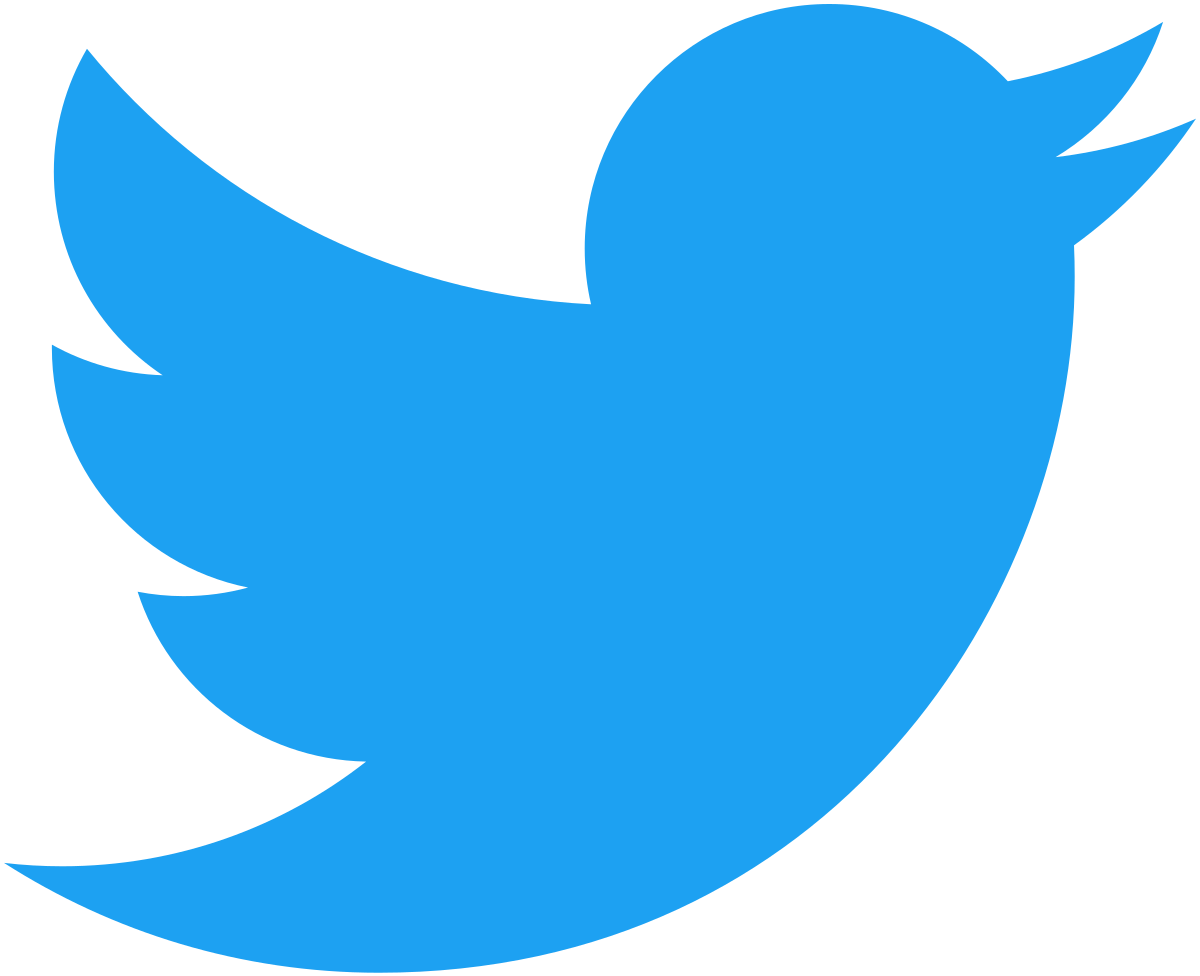
\includegraphics[scale=0.007]{./img/tw_logo.png}  &  \href{https://developer.twitter.com/en/docs/twitter-api/early-access}{Twitter API v2} & \multicolumn{1}{l|}{\href{https://github.com/medialab/minet/blob/master/docs/cli.md\#twitter-scrape}{Minet tw scrape}}                                                                                                                                                                           \\ \hline
 
\includegraphics[scale=0.03]{./img/yt_logo.png}  &  \href{https://developers.google.com/youtube/v3}{YouTube API v3}      &                                                                                                                            \multicolumn{1}{l|}{Code created for this article}                                                                                                                                                                           \\ \hline
\end{tabular}
\caption{Summary of ressources used for data collection.}
\label{tab1}
\end{table}

\smallskip

More specifically, we survey in this article a number of common policies against misinformation used by Facebook, Twitter and YouTube. We classified those common policies into three broad categories: $(i)$ temporary or permanent suspension of users, $(ii)$ 
informing users with flags and notices, and $(iii)$ reducing the visibility of some content. We compile in Appendix \ref{links} in table \ref{summary}, a list of links that redirect to the policies, regulations and transparency centers of Facebook, Twitter and YouTube that we discuss throughout the article. Furthermore, the examples provided to illustrate how to monitor a given policy were picked out of a list of domain names with several failed fact-checks. To be more precise, some domain names with failed fact-checks were picked because a given platform communicated about an intervention or because an intervention (e.g. suspension) was announced on the social media accounts linked to a given domain name. Finally, we discuss how an increased effort of transparency regarding specific content can help the community of researchers study and assess the impact of platforms' policies regarding misinformation. 

\smallskip 



%\bigskip

%{\color{red} Policies not specific to misinformation, but to enforce laws + things already used for terrorism and hate speech. Intro or/and Discussion. accounts: hard to say suspension for which.} 
% Misinformation : which law ? not defined ! 
%: Public content insights tool owned and operated by Facebook.
%\footnote{Public content insights tool owned and operated by Facebook.}
%: commercial content \\ database




 %We We are aware that other APIs or databases can be useful on that matter, but we will only mention here the ones about which we have some experience.
%CrowdTangle is a public insights tool owned and operated by Facebook, that exclusively tracks public content from Facebook public groups and pages. BuzzSumo is a commercial content database that tracks the volume of user interactions with internet content on Facebook, Twitter, and other social media platforms. 
%Section 230 in the US + EU 
%Pressure to moderate and mix-up of platforms with public square… 
%Rôle dans la production/médiation : P-M-R 
%Pourquoi faut-il vérifier leurs politiques ? D’une part parce que ce sont les plateformes elles-mêmes qui annoncent leurs effets. D’autre part beaucoup de choses indirectes. 
%Add disclaimer in a footnote early on in the document : document not meant to be an exhaustive overview of all the existing regulations and point to three or four main legal sources for exhaustive references. 
%Such policies include the introduction of notices (Twitter, see link) or flags (Facebook, see…) to signal to users inaccurate or false content, the temporary or permanent suspension of accounts (Twitter) or pages (Facebook), reducing the visibility of posts or pages (Facebook), or blocking users from sharing specific URL links (see link). The objective of this article is twofold. First, we study the impact of a number of  implemented measures by mainstream platforms to tackle (mis)disinformation. 


\section{Temporary \& permanent suspension}

Mainstream social media platforms may suspend the account of a specific user when they deem that the platforms' rules have been violated. Account suspension can be temporary or permanent.  When the suspension is temporary the user is prohibited for a limited period of time from posting content on their account, but 
content created prior to suspension remains available to the user and their followers. However, when the suspension is permanent, in most cases, followers or subscribers 
no longer have access to the content prior to the suspension and the user can no longer use the account to create new content. In what follows, we focus on the implementation of this policy by Facebook, Twitter and YouTube, and we provide simple examples to illustrate. 

\subsection{Facebook}

When an account is permanently suspended by Facebook, it disappears from the platform. That is,  the data can no longer be scrapped and it also disappears from the CrowdTangle API.\footnote{CrowdTangle is a public insights tool owned and operated by Facebook, that exclusively tracks public content from Facebook public groups and pages.} Facebook publishes on monthly basis a {\it coordinated inauthentic behavior} report, where it informs how many personal accounts, pages or groups were deleted and to which {\it deceptive network} they may have belonged to.\footnote{See the \href{https://about.fb.com/news/2021/05/april-2021-coordinated-inauthentic-behavior-report/}{April 2021 report} as an example.} 
But as long as external persons do not have access to historical data of deleted accounts, these reports cannot be verified by the academic community, NGOs and journalists.

\begin{figure}[h]
	\centering
		%\begin{multicols}{1}
			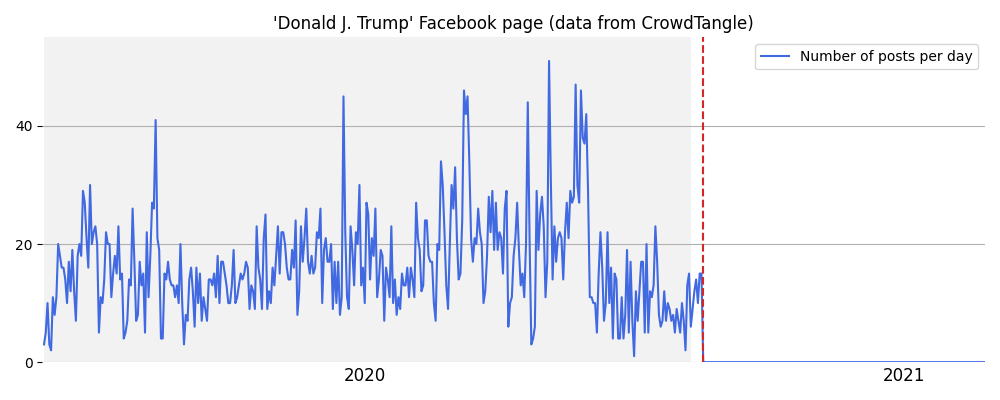
\includegraphics[scale=0.32]{../figure/facebook_crowdtangle_trump.png}
		%\end{multicols}
	\caption{Number of Facebook posts published each day by the Facebook page {\it Donald J. Trump} between January $1$, $2020$ and June $15$, $2021$. The data corresponds to $6$ $083$ posts retrieved from the CrowdTangle API using the {\it posts} endpoint.}
	\label{fig1_fb}
\end{figure}

Facebook can also apply a temporary suspension, and in this case the data can often be collected and analyzed. For example, \href{https://www.facebook.com/DonaldTrump/}{Donald Trump’s official Facebook page}  has been suspended following the Capitol attack on January 6, 2021.\footnote{See \href{https://www.facebook.com/zuck/posts/10112681480907401}{https://www.facebook.com/zuck/posts/10112681480907401}} Nevertheless the page’s data is still present in the CrowdTangle API. 
%Thus, after manually adding this page to the CrowdTangle dashboard, 
Hence, we collected the $6$ $083$ posts it had published between January $1$, $2020$ and June $15$, $2021$ using the {\it posts} endpoint.\footnote{See the endpoint documentation for more details: \href{https://github.com/CrowdTangle/API/wiki/Posts}{https://github.com/CrowdTangle/API/wiki/Posts}.} We used Minet command line tool \cite{minet} to collect the data. We can verify on figure \ref{fig1_fb} that the {\it Donald J. Trump} page has not published any content since January $6$, 2021, and that this behavior is not consistent with the page’s previous activity: an average of $16$ posts were published each day on Facebook before the suspension. 

\subsection{Twitter}

%paragraph strike system + say following example is a manual decision. 
Twitter has implemented a strike system as part of their Civic Integrity Policy and their COVID-19 misleading information policy. Violations of both policies can entail strikes, where two strikes lead to a 12-hour account lock and five or more strikes lead to permanent suspension from the platform. A list of notable Twitter temporary and permanent suspensions can be found on  \href{https://en.wikipedia.org/wiki/Twitter_suspensions}{Wikipedia}.\footnote{See \href{https://en.wikipedia.org/wiki/Twitter\_suspensions}{https://en.wikipedia.org/wiki/Twitter\_suspensions}.}
The 12-hour account lock is hard to observe in the data, 
especially for users who do not have an over the clock regular tweeting activity.\footnote{The following tool \href{https://makeadverbsgreatagain.org/allegedly/}{https://makeadverbsgreatagain.org/allegedly/} provides an overview of the daily and hourly tweeting activity, including repetition of Tweets for any given Twitter account.} 
In this section, we provide one example of a temporary suspension of a Twitter account, that seems to be the result of a manual decision concerning a Tweet which violated the rules. 

The Twitter account $@LifeSite$ of the website lifesitenews.com has been suspended for at least two periods of time: from end of 2019 until fall 2020 for 308 days, then again since January 2021 for having violated Twitter Rules\footnote{See Lifesitenews's article discussing the reason for the suspension: \href{https://www.lifesitenews.com/news/lifesite-is-dumping-twitter-and-so-should-you}{https://www.lifesitenews.com/news/lifesite-is-dumping-twitter-and-so-should-you}. Twitter rules can be found at: \href{https://help.twitter.com/en/rules-and-policies/twitter-rules}{https://help.twitter.com/en/rules-and-policies/twitter-rules}. }. In particular, this website has several failed fact-checks concerning the published articles, according to Iffy.news and feedback.org.\footnote{See \href{https://mediabiasfactcheck.com/life-site-news/}{https://mediabiasfactcheck.com/life-site-news/} and \href{https://open.feedback.org/media/S4}{https://open.feedback.org/media/S4}.}. We collected the activity (tweets, replies, quotes, retweets) on their Twitter account via the Twitter API, using the historical search endpoint. We then plotted the number of Tweets, Retweets, Quotes and Replies per day, as shown in panel $a$ of figure \ref{fig2}). The two periods of temporary suspension are clearly observed in the data as the user(s) of the account were not allowed to use the functionalities of the Twitter Platform. 

\begin{figure}[h]
\hspace{-2em}
%\centering
	%\begin{multicols}{1}
		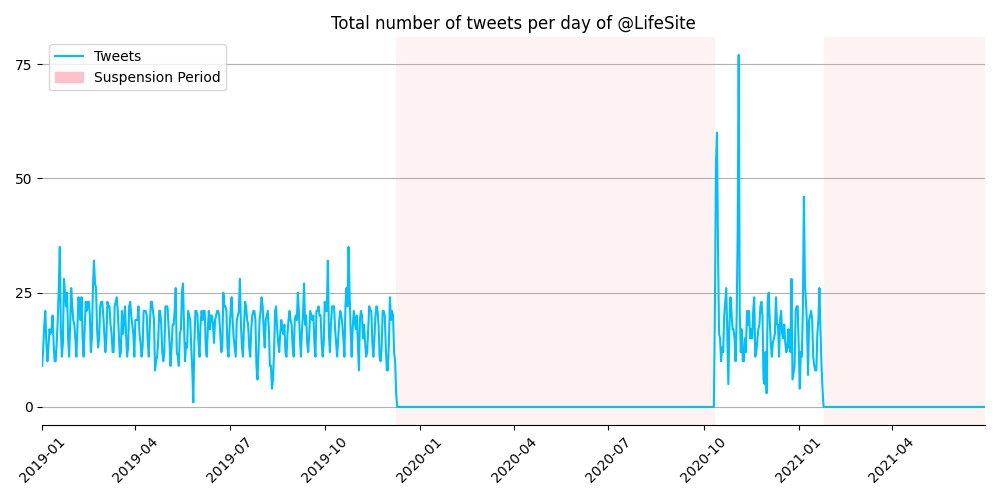
\includegraphics[scale=0.32]{../figure/lifesite.jpg} 
	%\end{multicols}
	%\begin{multicols}{1}
		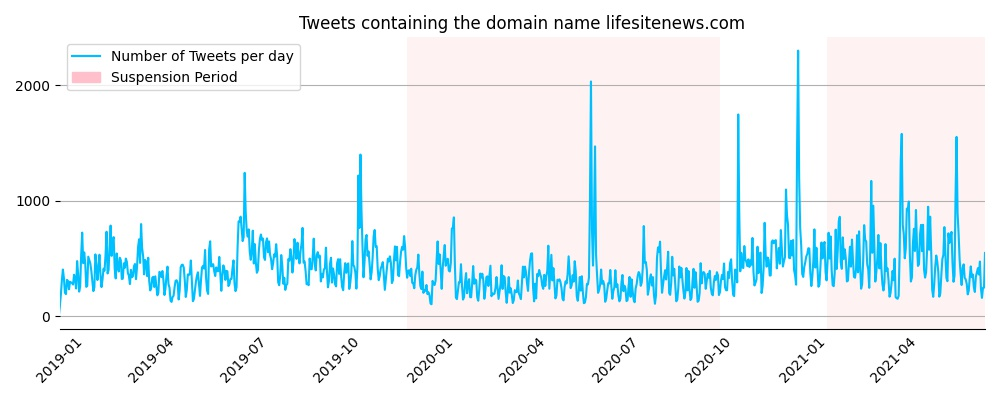
\includegraphics[scale=0.32]{../figure/lifesite_domain.jpg}
	%\end{multicols}
\caption{Left Panel: number of Tweets per day of the Twitter account $@Lifesite$ linked to the website lifesitenews.com from January, 2019 until April 2021. Right Panel: number of Tweets per day that have shared a lifesitenews.com URL link from January, 2019 until April 2021. }
\label{fig2}
\end{figure}

To further assess the impact of this double temporary suspension, we collect via the Twitter API v2, all the tweets that have shared during the same period a url link containing lifesitenews.com. Panel $(b)$ of figure \ref{fig2}, shows that during both periods of temporary suspension, other users still shared lifesitenews.com links and that the level was only slightly below the tweeting and retweeting levels prior to the first temporary suspension. More specifically, there was an average of 960 tweets (including retweets) per day over the first temporary suspension period of 308 days from December 9, 2019 until October 12, 2020, against an average of 977 tweets (including retweets) per day during the exact same period one year earlier. 

Finally, suspending a Twitter account is an intervention which aims at penalizing users, in order to make them respect the Twitter rules. In the case of Twitter accounts linked to domain names, the activity of the account usually consists in spreading on social media published articles on the website. Panel $(b)$ points towards the limitations of suspending the Twitter account $@LifeSite$, because the 
articles published on lifesitenews.com were still being actively shared by other Twitter users.

\subsection{YouTube}

In this section, we turn to the channel's temporary or permanent suspension policy of YouTube. 
When a YouTube channel violates the community guidelines, it can receive one or several strikes.
%Whenever a channel publishes a video that violates the community guidelines for the first time they will  usually receive a warning and the content will be removed. For the second time the channel will start receiving strikes. 
A first strike results in limiting the access of the YouTube channel for one week
(e.g. video uploading). 
Then a second strike is similar but the suspension lasts two weeks. 
A third strike results in the termination of the channel. 
The strike count of a channel lasts 90 days.  
In the special case, where a video is in extreme violation of the guidelines, the publishing channel may get terminated without a warning. 

\smallskip

\begin{figure}[h]
	\centering
	
	%\begin{multicols}{1}
		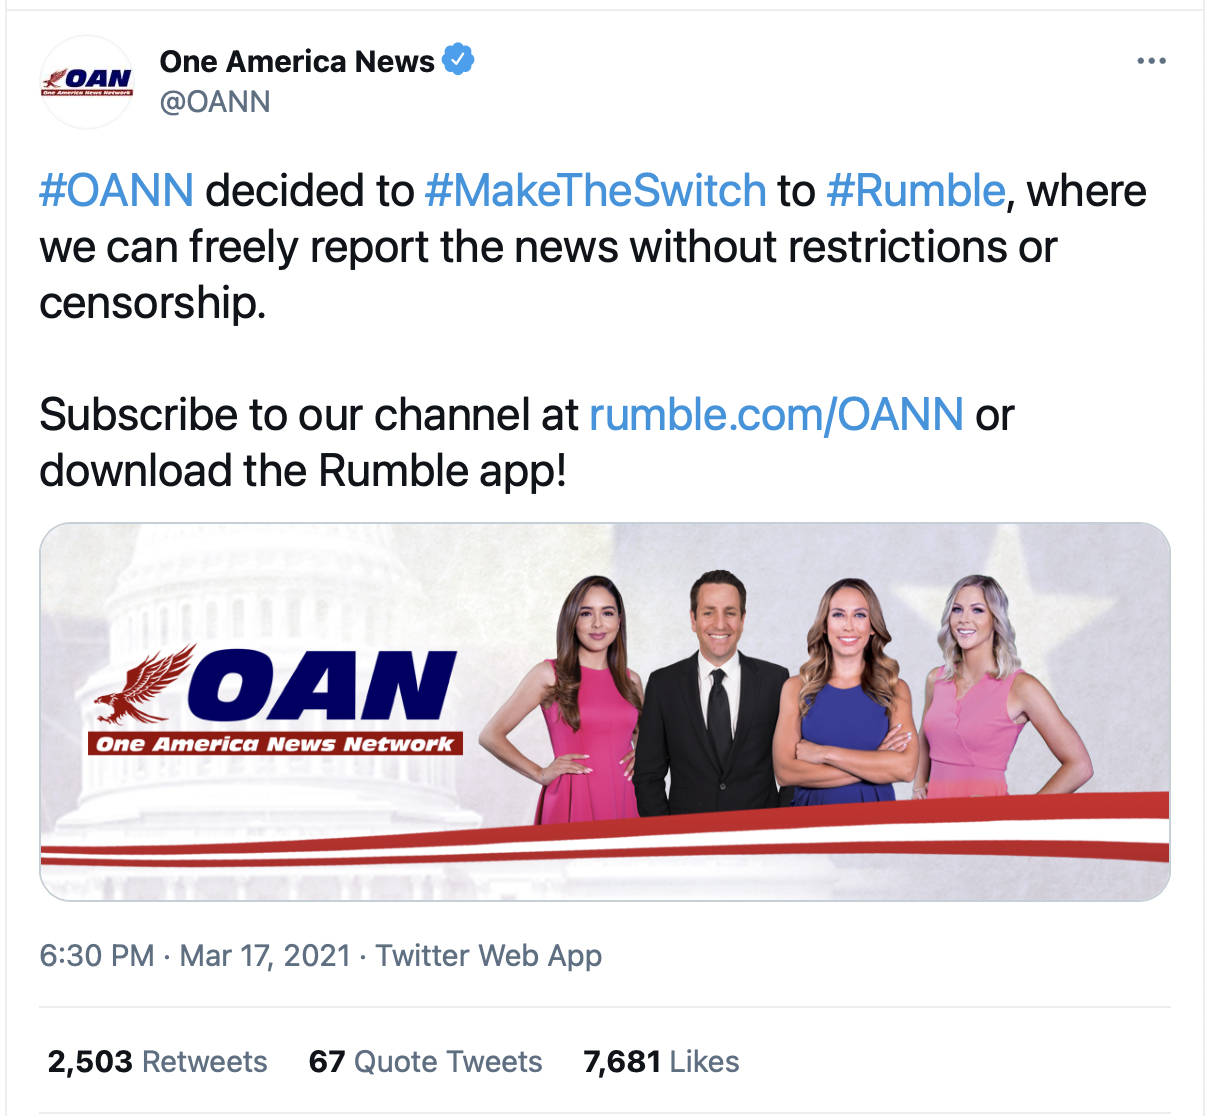
\includegraphics[scale=0.21]{./img/oann/fig3_oann.png}
	%\end{multicols}
	%\begin{multicols}{1}
		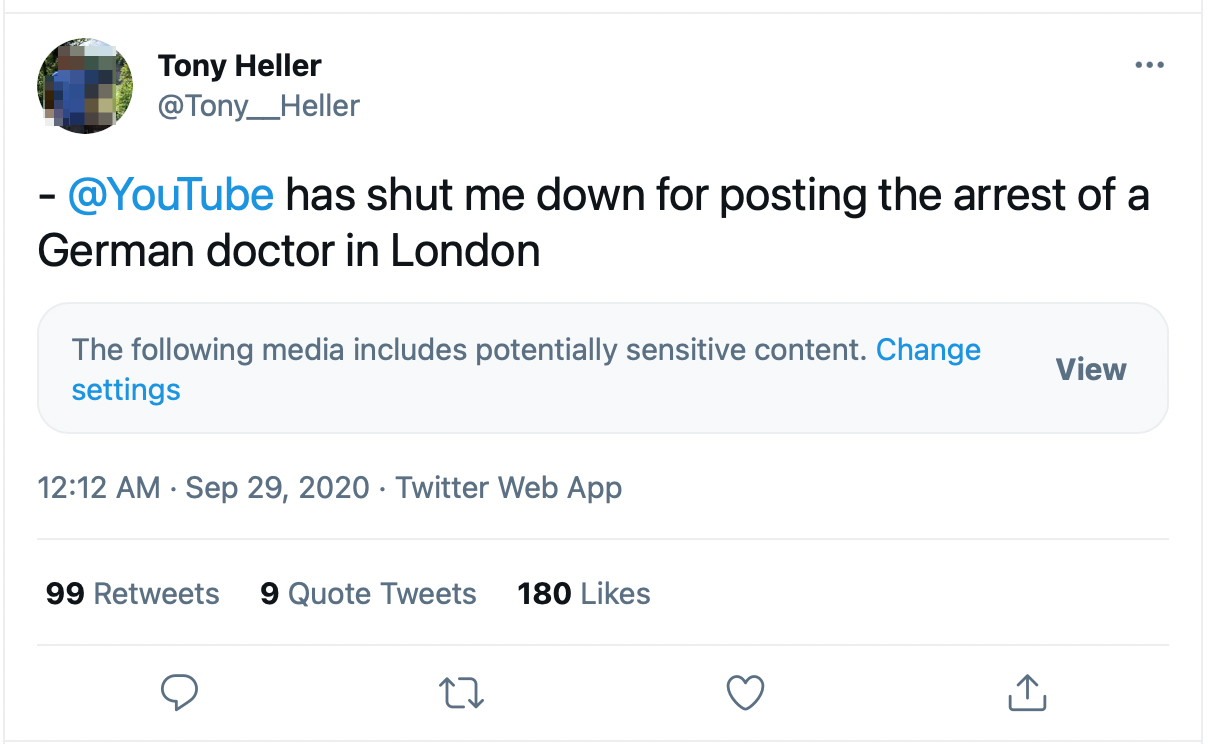
\includegraphics[scale=0.31]{./img/tony/fig3_tony.png}
	%\end{multicols}
	\caption{Left Panel: Tweet announcing moving to Rumble by OANN (Twitter), Twitter ID \href{https://twitter.com/OANN/status/1372238828425998336}{1372238828425998336}. Right Panel: Tony Heller's tweet after getting suspended from YouTube, Twitter ID \href{https://twitter.com/Tony\_Heller/status/1310703852769796097}{1310703852769796097}.}
	\label{fig2_oann}
\end{figure}

To illustrate the implementation of this policy we provide two examples for the temporary suspension of the following YouTube channels: \href{https://www.youtube.com/channel/UCNbIDJNNgaRrXOD7VllIMRQ}{One America news Network} and \href{https://www.youtube.com/user/TonyHeller1}{Tony Heller}. 
The website of One America News Network has a ``low'' factual reporting score according to iffy.news and several inaccurate articles according to feedback.org.\footnote{See \href{https://mediabiasfactcheck.com/one-america-news-network/}{mediabiasfactcheck.com/one-america-news-network/} and \href{https://open.feedback.org/media/AE6Q}{https://open.feedback.org/media/AE6Q}.}  
Tony Heller posts regularly blog posts on the website {\it realclimatescience.com}, which also has a ``low'' factual reporting score according to iffy.news.\footnote{See \href{https://mediabiasfactcheck.com/real-climate-science/}{mediabiasfactcheck.com/real-climate-science/}} 
Both are active on YouTube and both have communicated via their Twitter account about restrictions applied by YouTube over their content (see figure \ref{fig2_oann}).

\smallskip

First, we investigate the temporary suspension of the YouTube channel of One America News Networks. According to the News outlet NBCnews (2020)~\cite{nbcnews}, this YouTube channel received a first strike on November $24$, $2020$ for the promotion of a false cure for COVID-19.
We collected the activity of the channel OANN (video counts and view counts) using the YouTube API v3, between November $2020$ and January $2021$. For the video counts, we used the {\it playlists} endpoint to retrieve the videos uploaded with their publishing date and for the view count we used the IDs of the videos we had from the playlists, then via the {\it videos} endpoint we retrieved the view counts on June $2021$.%\footnote{See the Google documentation  \href{https://developers.google.com/youtube/v3/docs/videos/list}{https://developers.google.com/youtube/v3/docs/videos/list} and \href{https://developers.google.com/youtube/v3/docs/playlists/list}{https://developers.google.com/youtube/v3/docs/playlists/list}} 

\smallskip

Figure \ref{fig1_oann} shows the daily number of videos uploaded by the channel, and its number of views. 
We can clearly see the suspension period in the data, as the number of published video is down to zero for one week after the strike on November $24$, $2020$. 
Because no videos were published during this period, the number of views were also nul.
When comparing one month before and after the suspension, the view count decreased by -73\%, indicating that the videos uploaded after the suspension were less popular. 
Furthermore, the activity of the channel was close to zero after March 2021, and OANN's Twitter account has announced their migration from YouTube to Rumble on March 17, 2021.

\begin{figure}[h]
\hspace{-2em}
	%\centering
		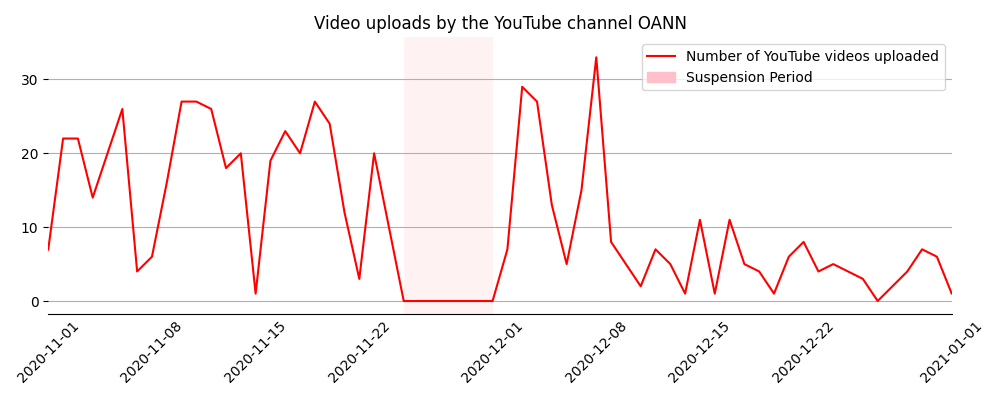
\includegraphics[scale=0.32]{../figure/delete_youtube_1_oann.png}
		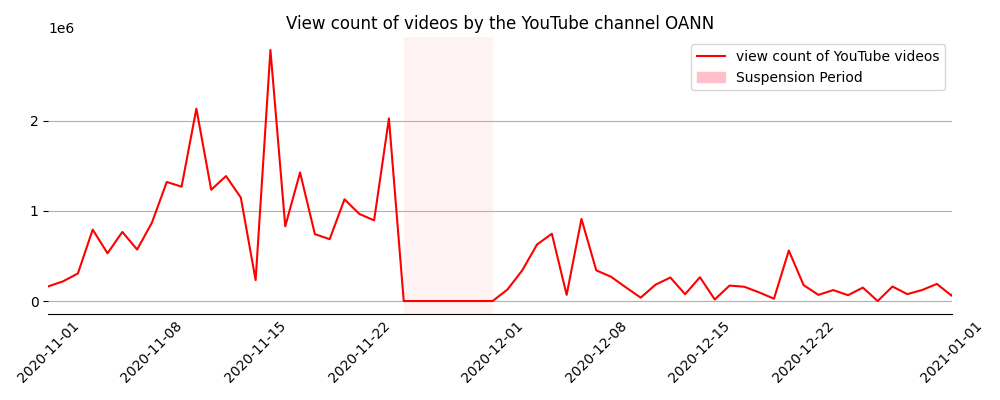
\includegraphics[scale=0.32]{../figure/delete_youtube_2_oann.png} 
	\caption{Left Panel: Number of YouTube videos uploaded each day by the youtube channel {\it One America news Network} November 1, 2020 and January 1, 2021. Right Panel: accumulated view counts for videos. The metrics correspond to the videos’  publishing date and the data is retrieved from the YouTube API with the {\it playlists} and  {\it videos} endpoints. }
	\label{fig1_oann}
\end{figure}

\smallskip

We now turn to a second example, the YouTube channel Tony Heller. 
This channel got its first strike after posting a video about an anti-covid-lockdown doctor getting arrested (see screenshot in figure \ref{fig2_oann}). 
The suspension period lasted one week from September $29$ until October $5$.
We applied the same methods as in the previous example to collect data.
Again the one-week suspension period can be observed clearly in the daily number of uploaded videos and of views.
Comparing one month before and after the suspension, this channel also witnessed a drop of view counts by $-70\%$.

\begin{figure}[h]
\hspace{-2em}
	%\centering
			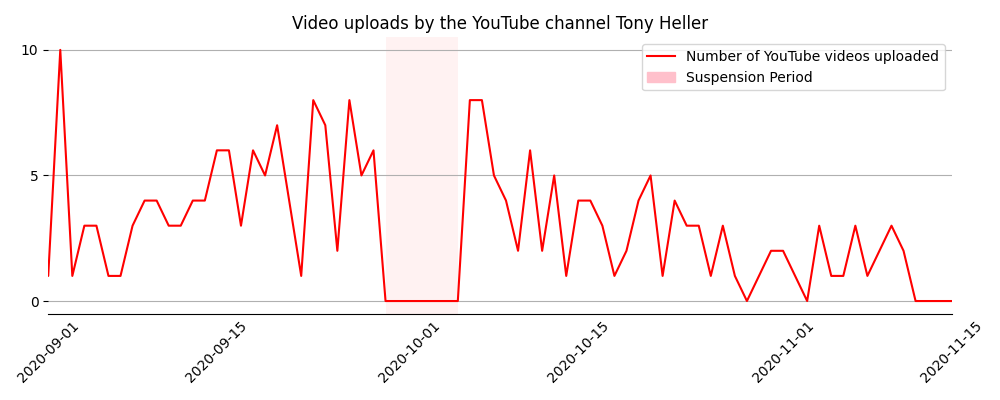
\includegraphics[scale=0.32]{../figure/delete_youtube_3_tony_heller.png}
			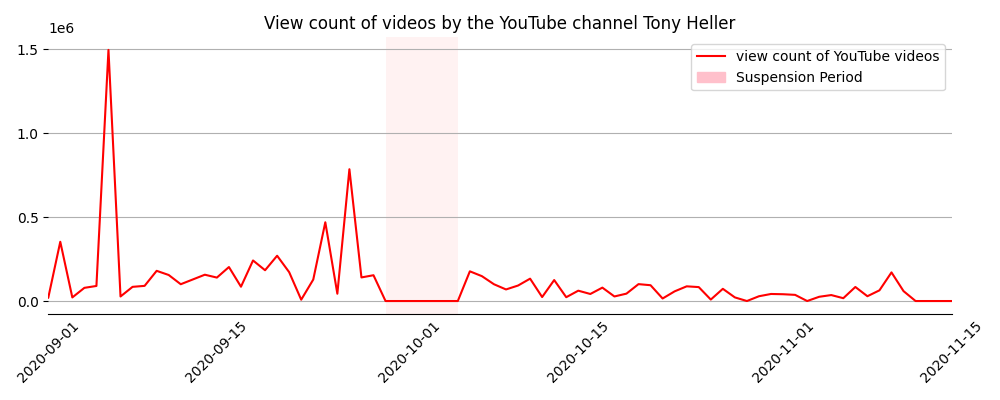
\includegraphics[scale=0.32]{../figure/delete_youtube_4_tony_heller.png}
	\caption{Left Panel: Number of YouTube videos uploaded each day by the YouTube channel {\it Tony Heller} between September 1, 2020 and November 15, 2020. Right Panel: accumulated view counts for videos uploaded by the same YouTube channel. The date corresponds to the videos’  publishing date. 
}
	\label{fig1_tony}
\end{figure}

As most YouTube channels upload videos on a weekly or even a monthly basis, a one-week suspension appears not very restrictive at first sight. 
But we observed that the intervention was followed by a reduction in the number of view for the two channels investigated, with one channel even stopping its YouTube activity in the following months. 
Although more research is needed before drawing a definitive conclusion, it is possible that the one-week suspension following a strike might reduce the reach of the very active YouTube channels.

%%%%%%%%%%%%%%%%%%%%%%%%%%%%%%%%%%%%%%%%%%%%%%%%%%%%%%%%%%%%%%%

\section{Flags, Notices and information panels} \label{flags}

Mainstream platforms such as Facebook, Twitter and YouTube can resort to providing more context to users regarding a specific post, Tweet or video. This type of intervention takes different formats according to the platform and also has different denominations. Facebook for example refers to this intervention by mentioning ``flags", while Twitter  refers to ``notices" and ``interstitials" and YouTube uses the term ``information panels". In this section, we explain the specifics of this intervention for each platform and illustrate with examples. 

\subsection{Facebook}

To the best of our knowledge, two types of flags can currently be displayed on Facebook posts: 
$(i)$ information banners which do not refute the message in the post and provide a link which redirects to an authoritative source, such as ``Visit the COVID-19 Information Centre for vaccine resources'' and $(ii)$ fact-check flags that assigns a ``rating" for a text or a link in a given post, such as ``False information Checked by independent fact-checkers'' (see Figure \ref{fb_flags}). The fact-check flags display the following ratings : ``False", ``Partly false", ``Missing context", ``False headline", ``Altered media", ``Opinion", ``Satire", ``Not eligible" and ``True".\footnote{See \href{https://www.facebook.com/business/help/341102040382165}{https://www.facebook.com/business/help/341102040382165}.}

\begin{figure}[h]
\centering
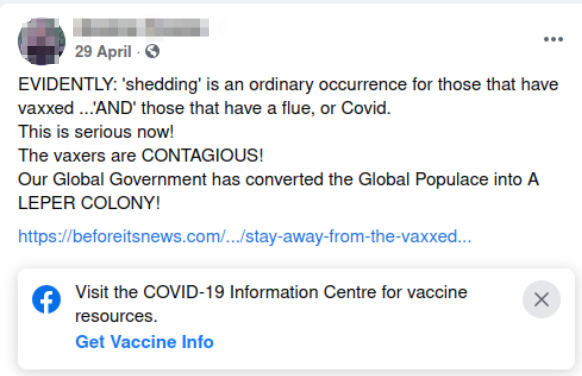
\includegraphics[scale=0.35]{./img/fb_flags/fb_flag_1.png}
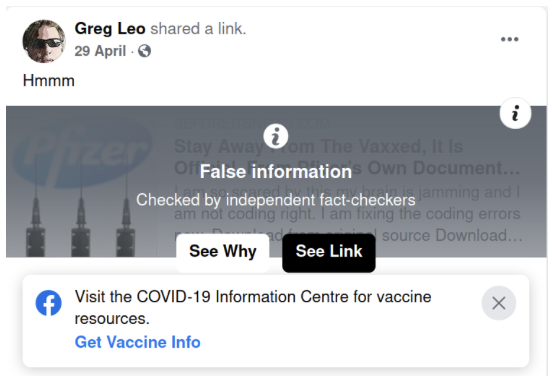
\includegraphics[scale=0.35]{./img/fb_flags/fb_flag_2.png}
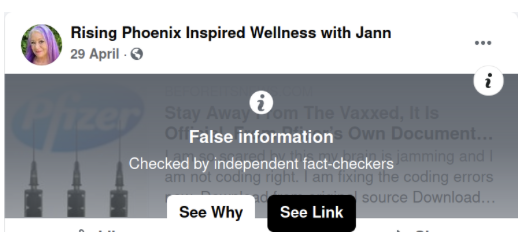
\includegraphics[scale=0.49]{./img/fb_flags/fb_flag_3.png}
\caption{Examples of Facebook posts having shared a link fact-checked as False by one of Facebook’s partners. Screenshots taken on July 8, 2021: \href{https://www.facebook.com/groups/1220117708132394/permalink/2386760061468147}{facebook.com/groups/1220117708132394/permalink/2386760061468147},  \href{https://www.facebook.com/groups/473809623000471/permalink/1333200093728082}{facebook.com/groups/473809623000471/permalink/1333200093728082}, \href{https://www.facebook.com/691911990845585/posts/3835629366473816}{facebook.com/691911990845585/posts/} \href{https://www.facebook.com/691911990845585/posts/3835629366473816}{3835629366473816} .} 
\label{fb_flags}
\end{figure}

No information or available fields regarding the Facebook flags can be found on Buzzsumo or CrowdTangle, the two APIs we use to access Facebook data. The only way to verify Facebook’s flagging policy is thus via scraping publicly available content. To that end, we added a new feature in Minet~\cite{minet} which could automatically verify the presence or absence of flags.

We first searched for all the Facebook posts having shared a specific link rated as ‘False’ by Science Feedback, a fact-checking organization which partners with Facebook. We used the {\it search} endpoint in Minet.\footnote{ Click \href{https://beforeitsnews.com/eu/2021/04/stay-away-from-the-vaxxed-it-is-official-from-pfizers-own-documents-2671454.html}{here} to access the link and  \href{https://healthfeedback.org/claimreview/insufficient-evidence-to-claim-covid-19-vaccines-cause-menstrual-irregularities-in-vaccinated-women-vaccinated-people-arent-making-unvaccinated-people-ill/}{its fact-check by Health Feedback}.} 
Twenty Facebook posts were collected this way, and the newly developed scraper was used to verify whether they contained an information banner, a fact-check flag, both or none. Three posts were unavailable, and thus could not be categorized by the scraper. As Science Feedback has informed Facebook that they have assigned the rating ``False'' for this link, we expected that all these posts would contain a fact-check flag, but we had no expectations for the information banner. 

\begin{table}[h]
\begin{tabular}{|c|c|c|c|}
\hline
\multicolumn{4}{|c|}{Number of posts}                                                                                                                    \\ \hline
without a flag & with an information flag & with a fact-check flag & \begin{tabular}[c]{@{}c@{}}with a fact-check and an \\  information flags\end{tabular} \\ \hline
0            & 7                        & 4                      & 7                                                                                     \\ \hline
\end{tabular}
\caption{Count for the Facebook posts with the different types of flags having shared a link fact-checked False by one of Facebook’s partners}
\label{tab_flags_fb}
\end{table}

\smallskip

Surprisingly only $11$ posts out of the remaining $17$ had a ``False information'' flag  (Table \ref{tab_flags_fb}, see left panel of Figure \ref{fb_flags} for an example). We observed that the flagged posts were also the ones in which the false link was expanded (i.e., a banner was visible with an image of the link and that can be clicked on, see the middle and right panels of Figure \ref{fb_flags} for examples). As the ‘False information’ flag is applied on the link banner, and not on the link itself, a user is thus able to share a ``False'' link on Facebook without the ``False'' flag if the link is not expanded.

\smallskip

We also observed that most of the posts sharing this ``False'' link (13 out of 17, Table \ref{tab_flags_fb}) had an information banner saying ``Visit the COVID-19 Information Centre for vaccine resources" (see the first two examples of Figure \ref{fb_flags}). We could not identify why the banner was applied on some posts and not on others (we saw no clear difference in the post messages for example). It should be noted that some posts displayed both the information and the fact-check banners, as in the middle panel of Figure \ref{fb_flags}.

\subsection{Twitter}

Alongside other social networking platforms, when the content of a tweet violates the Twitter rules, a notice can be added to provide more context according to Twitter's Help Center. At the tweet level, notices take the form of a label or an interstitial. Labels are context specific (e.g. COVID-19 or presidential elections) and  redirect users to a webpage to get more context, for example {\it ``Get the facts about COVID-19''} (see right panel of figure \ref{fig8}). Interstitials are presented as a greyed box on top of a tweet, which indicates sensitive content, violations of Twitter rules, withheld tweets for violation of local laws or even tweets from suspended accounts, for example {\it ``The following media includes potentially sensitive content''} (see left panel of figure \ref{fig_notice}). At the account level, notices can also indicate whether an account has been temporarily or permanently suspended. 

%\smallskip 

\begin{figure}[h]
\centering
	%\begin{multicols}{1}
		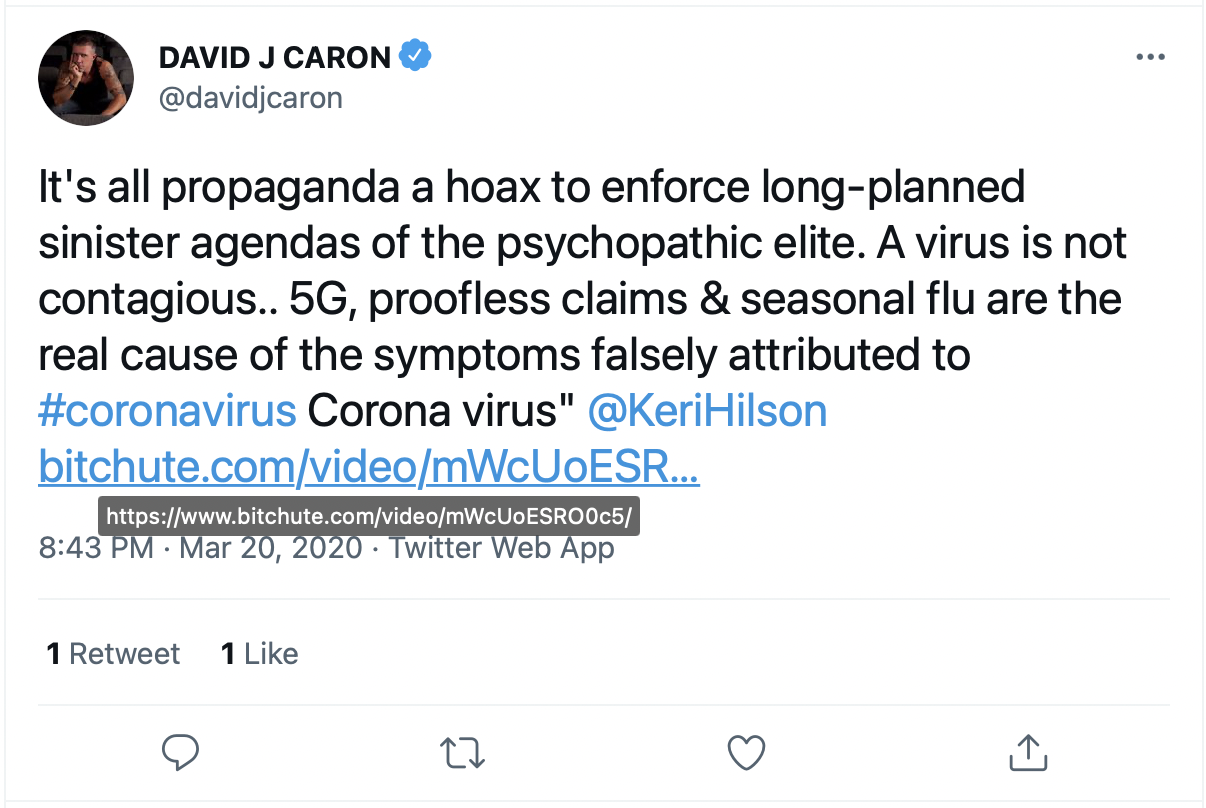
\includegraphics[scale=0.35]{./img/tweets/Capture_2021-06-30_2.png}
   	 %\end{multicols}
	%\begin{multicols}{1} 
		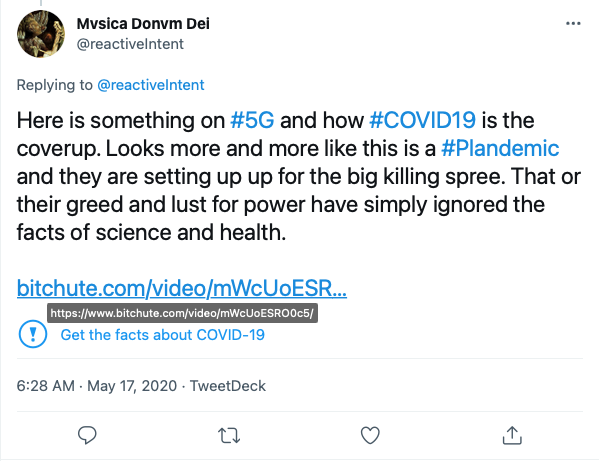
\includegraphics[scale=0.32]{./img/tweets/Capture_2021-06-30.png}
	%\end{multicols}
	\caption{Two tweets sharing the same link marked as ``False'' by Science Feedback, screenshots taken on June $20$, 2021. Left Panel: Tweet ID \href{https://twitter.com/davidjcaron/status/1241088065462026242}{1241088065462026242} without a label. Right Panel: Tweet ID \href{https://twitter.com/reactiveIntent/status/1261876171584745472}{1261876171584745472} containing a label.}
	\label{fig8}
\end{figure}

\smallskip

To the best of our knowledge, when using the Twitter API v2, there is no field which indicates whether a tweet contains a label or not; while the interstitial ``possibly sensitive'' and ``withheld" are both Tweet fields that can be recovered\footnote{See \href{https://developer.twitter.com/en/docs/twitter-api/data-dictionary/object-model/tweet}{https://developer.twitter.com/en/docs/twitter-api/data-dictionary/object-model/tweet}.} from the Twitter API v2. Hence, in order to investigate the presence of notices of all types, we resorted to scrape publicly available tweets, using Minet [5]. This tool was recently enriched upon our request in order to capture whether a tweet contains a notice or not, via the ``minet twitter scrape'' command.

\smallskip

In this section, we take a deeper look at how labels and interstitials are introduced by Twitter, to indicate content which is inaccurate or false. To that end, we gathered a set of $3$ $094$ links redirecting to articles which were marked as ``False'' between April $2019$ and February $2021$ by Science Feedback, a fact-checking organization verifying the credibility of science-related viral information. 
As a second step, we collected (on June $30$, $2021$) using Minet~\cite{minet} all the tweets that have shared a link which belongs to the set of $3$ $094$ links marked as $False$. This data collection resulted in $323$ $938$ tweets, excluding retweets. Only $28$ tweets contained the label { \it ``Get the facts about COVID-19''}, $5$ tweets contained the label {\it ``Learn about US 2020 election security efforts''} and only $1$ had the following label {\it ``This claim about election fraud is disputed''}. Furthermore, we noticed that the labeling rule might not be applied uniformly on a given set of tweets sharing the exact same link, among the set of collected tweets. To give an example, $657$ tweets had shared the exact same link redirecting to a video on Bitchute, entitled {\it Important information on coronavirus 5G Kung Flu}. Among those $657$ tweets only $3$ contained the label {\it ``Get the facts about COVID-19''} (see figure \ref{fig8}). This points towards the non-automation of the tweet labelling process and that it might be that these $3$ tweets were the only ones reported by other users. 

\begin{figure}[h]
	\centering
	%\begin{multicols}{1}
		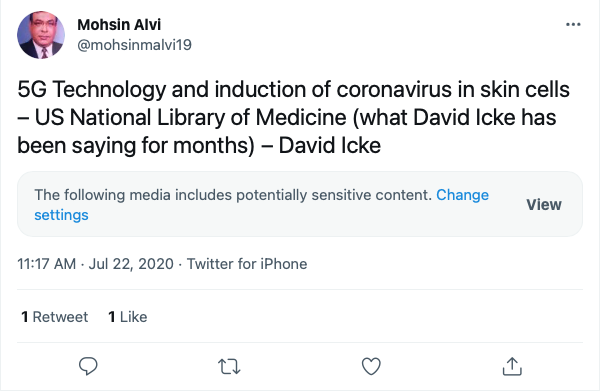
\includegraphics[scale=0.35]{./img/tweets/Capture_2021-07-01_2.png} 
	%\end{multicols}
	%\begin{multicols}{1}
		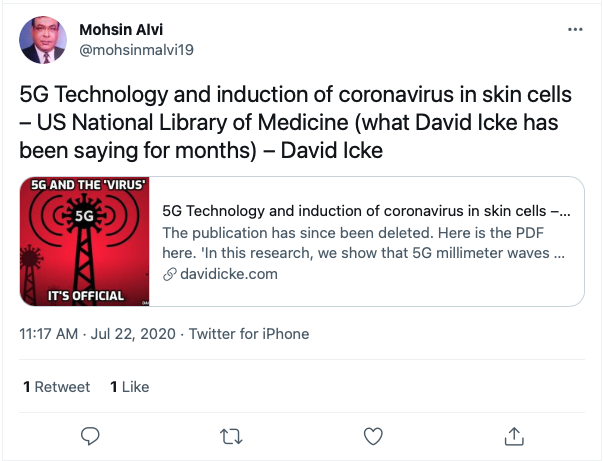
\includegraphics[scale=0.35]{./img/tweets/Capture_2021-07-01.png}
	%\end{multicols}
	\caption{Left Panel: Tweet containing a URL link hidden behind an interstitial. Right Panel: when clicking on $view$, to view the content hidden behind the interstitial in the left panel. Tweet ID \href{https://twitter.com/mohsinmalvi19/status/1285866521533861888}{1285866521533861888}. Screenshots taken on July 1, 2021. }
	\label{fig_notice}
\end{figure}

\smallskip

We further examine the placement of interstitials that indicate a possibly sensitive content. We find that only $9$ $344$ ($2.97\%$) tweets out of $323$ $938$ containing a link marked as False, have an interstitial {\it ``potentially sensitive content''}. To check whether the interstitial {\it ``potentially sensitive content''} is automated or not, we pick out one tweet having shared a link\footnote{The link marked as False redirects to the article {\it 5G Technology and induction of coronavirus in skin cells – US National Library of Medicine (what David Icke has been saying for months) } and can be found \href{https://davidicke.com/2020/07/22/5g-technology-and-induction-of-coronavirus-in-skin-cells-us-national-library-of-medicine-what-david-icke-has-been-saying-for-months/}{here}.} marked as ``False'', which also contains the interstitial {\it potentially sensitive content} (see figure \ref{fig_notice}). Then we look in the set of $323$ $938$ tweets for other tweets who have shared the exact same link. We find a total of $32$ tweets. Among those $32$ tweets only $5$ tweets had the interstitial ``potentially sensitive content''. Again this points towards the non-automation of interstitials placement. Furthermore, notice that the appearance of interstitials may depend on the settings of a user's account and country or language specific regulations. In particular, in the settings of Twitter account, one can deactivate the display of interstitials for {\it sensitive content}, by ticking the box {\it Display media that may contain sensitive content} in the section {\it content you see}. 

\smallskip

Finally, the number of tweets containing the interstitial {\it ``potentially sensitive content''} ($9$ $344$ tweets) widely outnumbers the tweets which contain a flag ($32$ tweets), among the set of $323$ $938$ tweets containing a link marked as ``False'' (see table \ref{flags_tab}). Furthermore, we noticed that among the tweets which contain the interstitial {\it ``potentially sensitive content''}, there are tweets which contain links redirecting to misleading articles about COVID-19 and yet they do not contain the label { \it ``Get the facts about COVID-19''}. We also noticed that the $9$ $344$ tweets which contain the interstitial {\it ``potentially sensitive content''} do not necessarily contain graphic violent content\footnote{The Twitter Help center explains the placement of interstitials of possibly sensitive content as follows: ``We may place some forms of sensitive media like adult content or graphic violence behind an interstitial advising viewers to be aware that they will see sensitive media if they click through''.} but rather links that redirect to articles marked as ``False'' by Science Feedback. When navigating through the Twitter Help Center, we found no explanation for this large discrepancy between using the interstitial {\it ``potentially sensitive content''} and labels which provide more context to users.\footnote{Twitter Safety account announced in a Tweet (see Tweet ID : \href{https://twitter.com/TwitterSafety/status/1379515615954620418}{1379515615954620418}) on April 6, 2021 that their team ``will begin deploying automated tools to build on (their) efforts to label tweets that may contain misleading information around COVID-19 vaccinations".}  

\begin{table}[h]
\centering
\begin{tabular}{|c|c|c|c|}
\hline
\multicolumn{4}{|c|}{$323$ $938$ Tweets containing a link marked as False}                                                                                                                                                                                                                                                                                                                           \\ \hline
\begin{tabular}[c]{@{}c@{}}with the interstitial\\ ``potentially sensitive \\ content'' \end{tabular} & \begin{tabular}[c]{@{}c@{}}with the flag \\ ``Get the facts \\ about COVID-19'' \end{tabular} & \begin{tabular}[c]{@{}c@{}}with the flag \\ ``Learn about US \\ 2020 election \\ security efforts'' \end{tabular} & \begin{tabular}[c]{@{}c@{}}with the flag\\ ``This claim about \\ election fraud \\ is disputed''\end{tabular} \\ \hline
\begin{tabular}[c]{@{}c@{}}9344\\ (2.88450 \%)\end{tabular}                                  & \begin{tabular}[c]{@{}c@{}}28\\ (0.00864 \%)\end{tabular}                              & \begin{tabular}[c]{@{}c@{}}5\\ (0.00154 \%)\end{tabular}                                                & \begin{tabular}[c]{@{}c@{}}1\\ (0.00030 \%)\end{tabular}                                             \\ \hline
\end{tabular}
\caption{Summary of the number of tweets among the set of collected tweets containing a link marked as False by Science Feedback, which contain a flag or an interstitial.}
\label{flags_tab}
\end{table}

\subsection{YouTube} \label{youtube_panels}

YouTube provide information panel at the top of search results or under a video related to topics prone to misinformation.
Information panels provide more context on a controversial matter, with a link to an independent, third-party partner's website such as Wikipedia or the World Health Organization. 
Importantly, YouTube states that these panels exist regardless of the point of view expressed in a given video.\footnote{https://support.google.com/youtube/answer/9004474}

\smallskip

To further study the assignment of information panels to videos, we compiled a list of $170$ YouTube videos, fact-checked by Science Feedback between April $2019$ and March $2021$ and marked as containing false or inaccurate information. 
We collected the information panels, when present, under each video by connecting to a US server and scraping the content of the web page. 
Four types of information panels were found regarding climate change, COVID-19 Vaccine, COVID-19 and US elections, as shown in figure \ref{youtube_panel_screenshots}.

\begin{figure}[h]
	\centering
		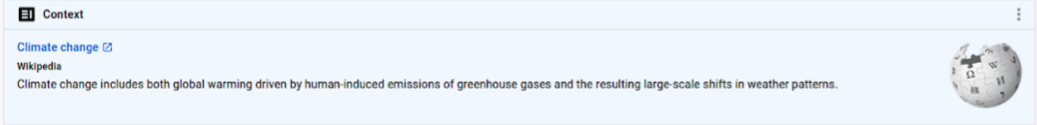
\includegraphics[scale=0.3]{./img/youtube_panels/yt_1.png} 
		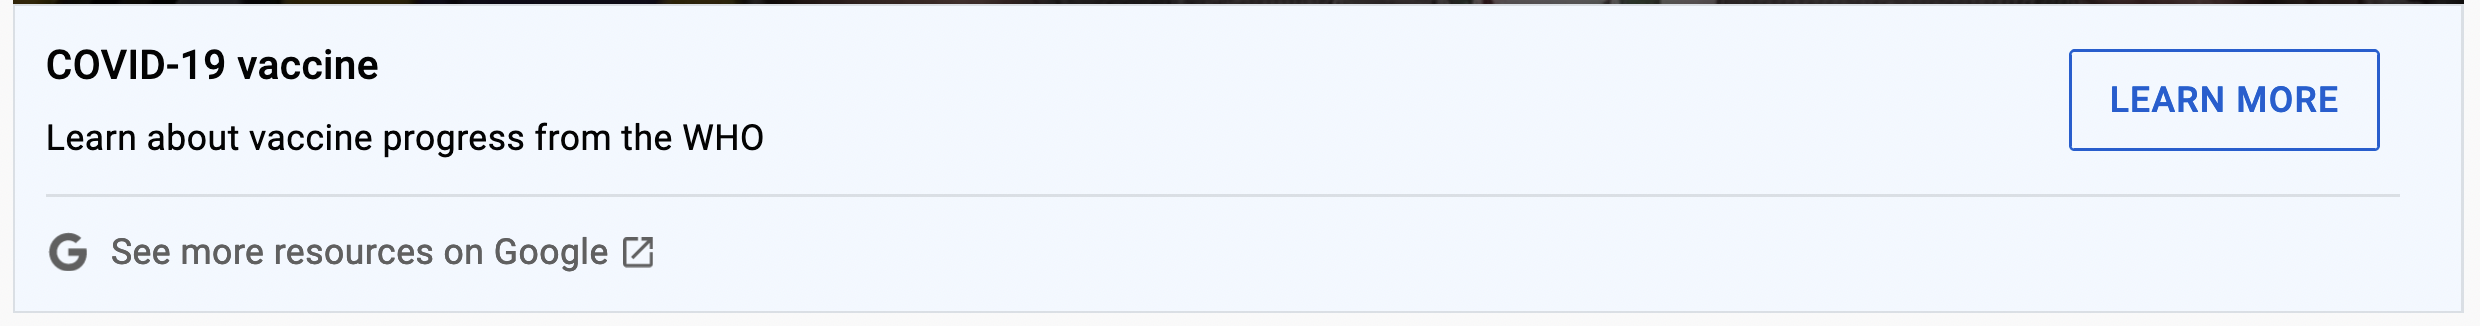
\includegraphics[scale=0.29]{./img/youtube_panels/yt_2.png} 
		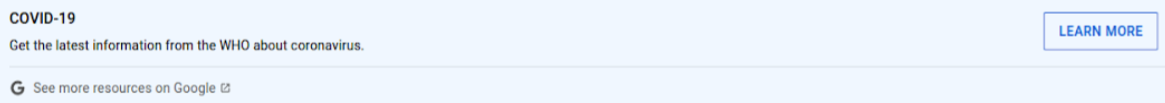
\includegraphics[scale=0.294]{./img/youtube_panels/yt_3.png}
		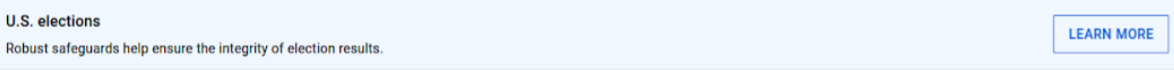
\includegraphics[scale=0.3]{./img/youtube_panels/yt_4.png} 
	\caption{Examples of YouTube information panels displayed under Youtube videos respectively about: \href{https://www.youtube.com/watch?v=OwqIy8Ikv-c}{Climate change}, \href{https://www.youtube.com/watch?v=9sW0OmzcmL0}{COVID-19 Vaccine}, \href{https://www.youtube.com/watch?v=usyQgPU-VrI}{COVID-19} and \href{https://www.youtube.com/watch?v=8PAwc8nlE\_Q}{US elections}. The videos were accessed on July 21, 2021 from a US server.}
	\label{youtube_panel_screenshots}
\end{figure}


\begin{table}[h] 
\centering
\begin{tabular}{|c|c|c|c|c|}
\hline
\multicolumn{5}{|c|}{$170$ YouTube videos marked as false or inaccurate}                                                                                                                                                                                                                                                                                                                           \\ \hline
\makecell{Without \\ any \\ panel} & 
\makecell{With a \\ `COVID-19' \\ panel} & 
\makecell{With a \\ `COVID-19 vaccine' \\ panel} &
\makecell{With a \\ `climate change' \\ panel} &
\makecell{With a \\ `U.S. elections' \\ panel}  
\\ \hline
\makecell{75 \\ (44 \%)} &
\makecell{71 \\ (42 \%)} &
\makecell{19 \\ (11 \%)} &
\makecell{4 \\ (2 \%)} &
\makecell{1 \\ (0.6 \%)}
\\ \hline
\end{tabular}
\caption{Summary of the number of YouTube videos wich contain a certain information panel, among the set of videos marked as false or inaccurate by Science Feedback.}
\label{youtube_panel_proportions}
\end{table}

\smallskip

Almost half (44 \%) of the videos containing misinformation were shown without any information panel (Table \ref{youtube_panel_proportions}).
For the rest of videos, the most frequent information panels concerned COVID-19 (42 \%) and COVID-19 vaccine (11 \%).
It is possible that YouTube is currently focusing its efforts on the current `hot' controversial topics with a potentially wide public impact, leaving room for misinformation related to other topics to spread, but more research is needed to formally compare misinformation videos about COVID-19 and about other subjects.

\smallskip

We noticed that the same video was sometimes uploaded multiple times and thus appeared on different YouTube links. 
One YouTube link might contain an information panel while its duplicates did not (see figure \ref{duplicates_yt} for an example).  
In addition, we noticed that some keywords in the video titles were often associated with an information panel, such as `COVID-19', `coronavirus', `pandemic' and `testing', while some notational variants like `C O V I D 19' or `Cv19' were not associated with a panel.
Therefore, we suspect that YouTube is automatically adding information panels based on the presence of certain keywords in the video title (and maybe in the video description), independently of the content of the video.
Note that in figure \ref{duplicates_yt}, the video with `C.O.V.I.D.19' in its title had an information panel, hinting that YouTube might adapt its list of suspect keywords as new notational variants for COVID-19 appear, or that some information panels might be added manually (by content regulators or when a video is flagged by many users).

\begin{figure}[h]
	\centering
		\begin{multicols}{1}
		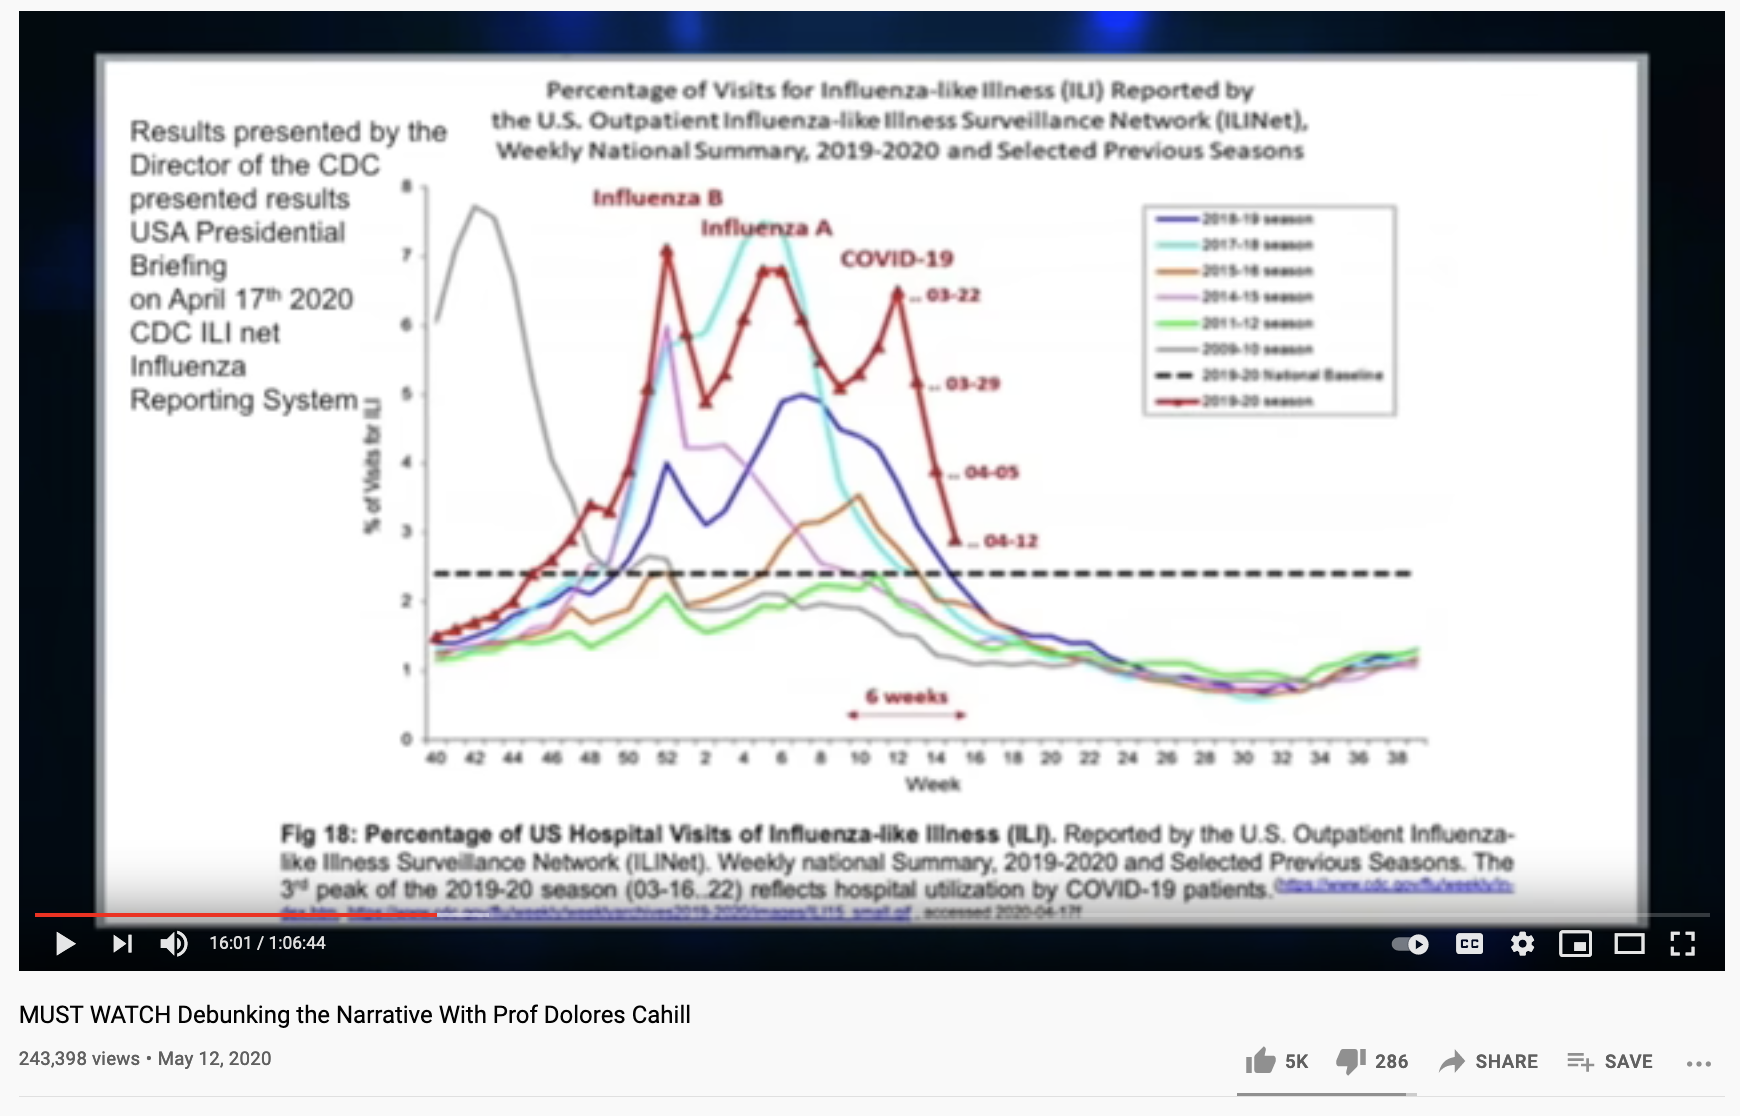
\includegraphics[scale=0.24]{./img/youtube_panels/graph_no_banner.png}
		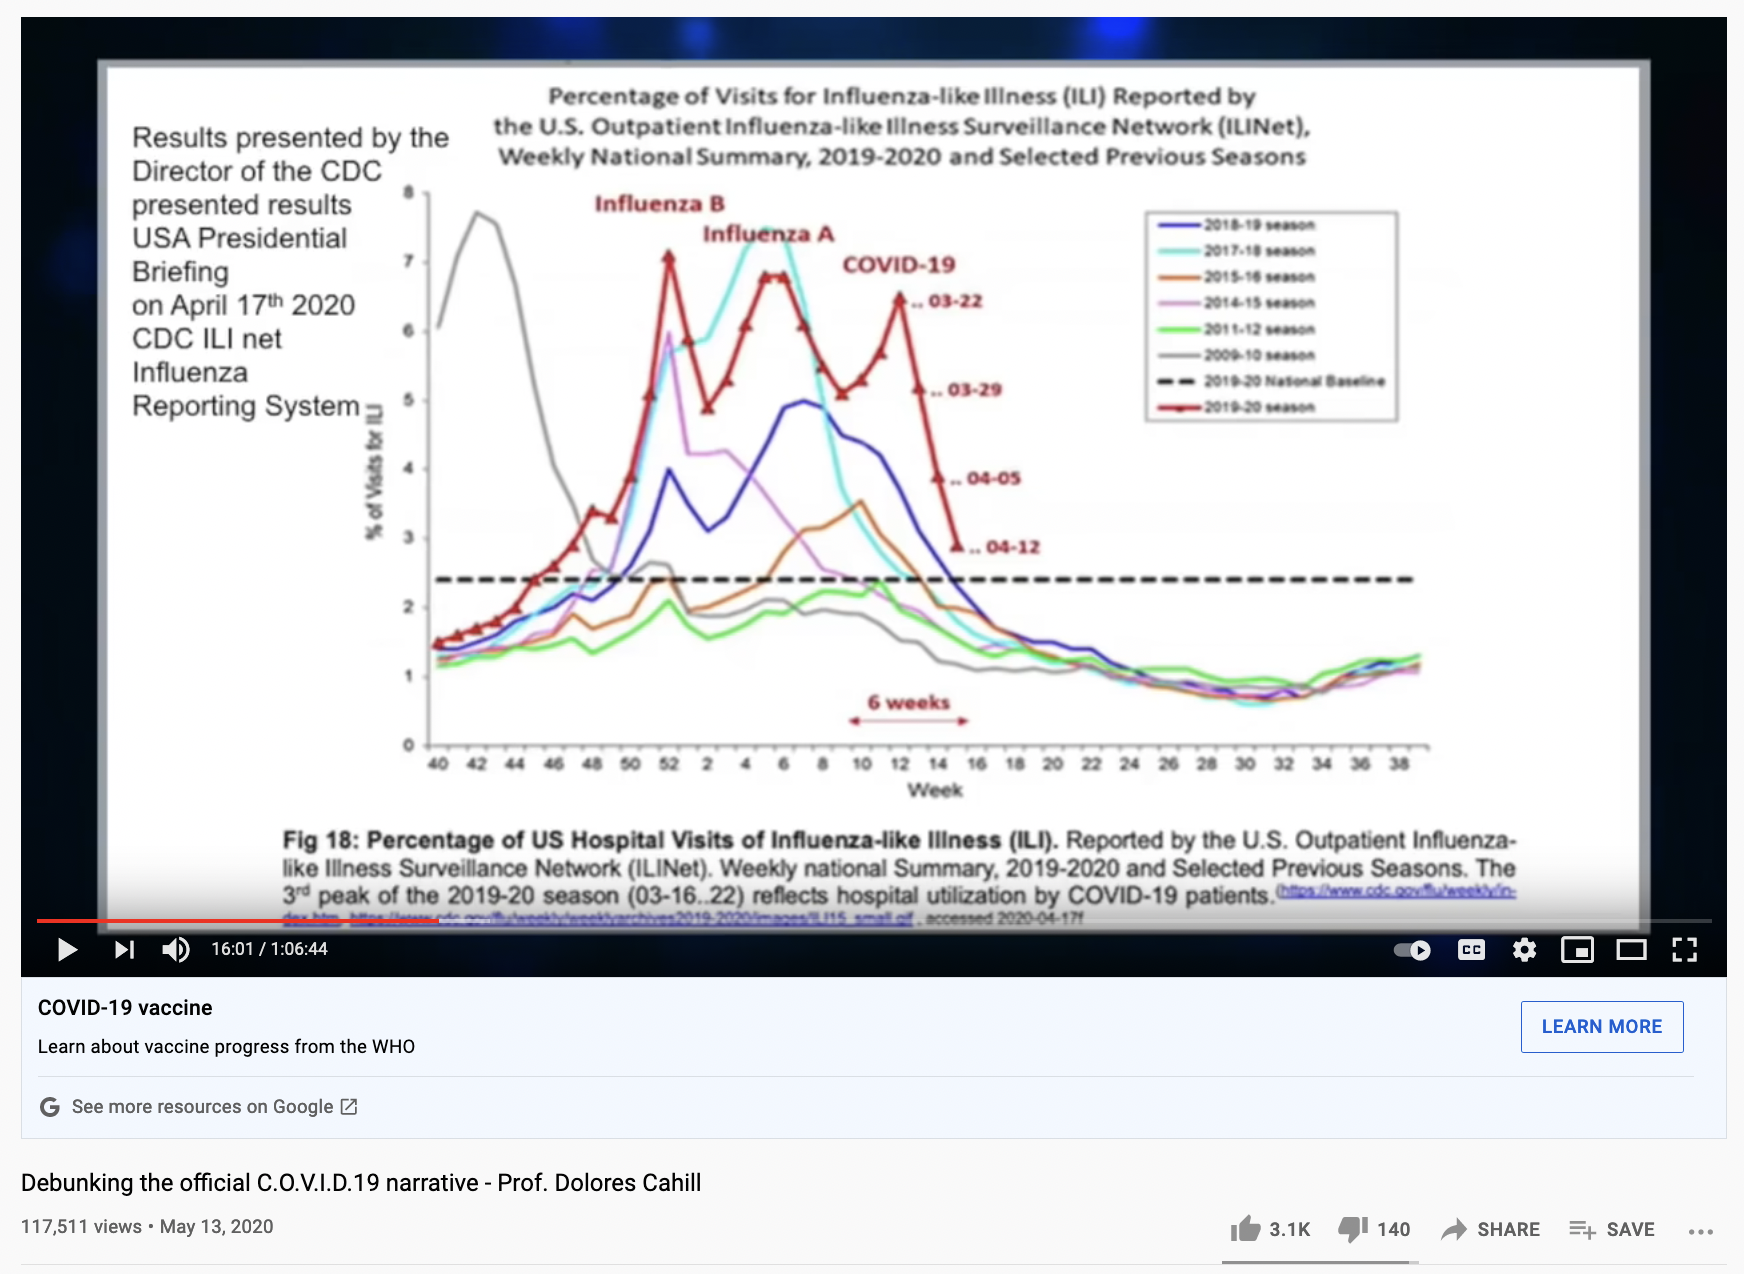
\includegraphics[scale=0.24]{./img/youtube_panels/graph_with_banner.png} 
		\end{multicols}
		%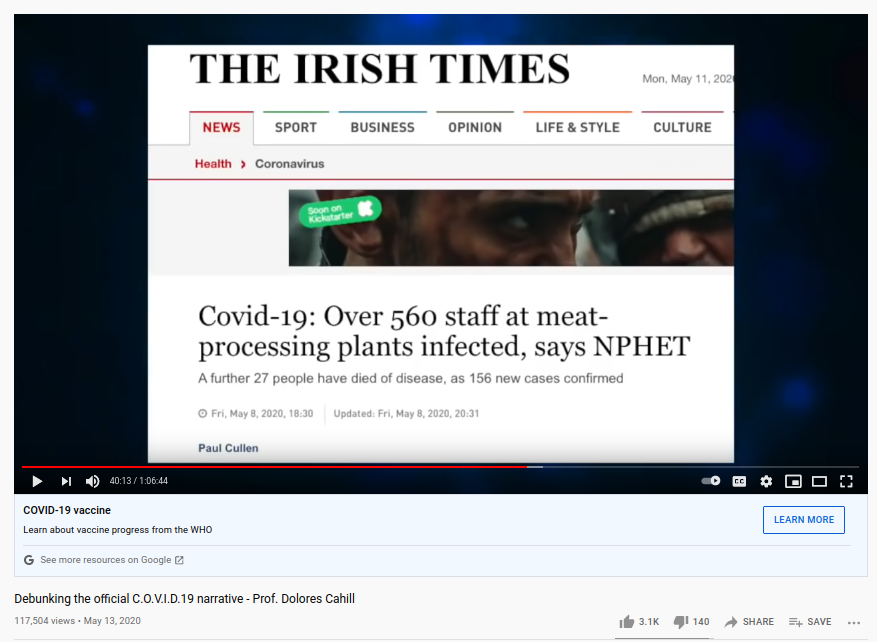
\includegraphics[scale=0.2]{./img/youtube_panels/news_with_banner.png}
		%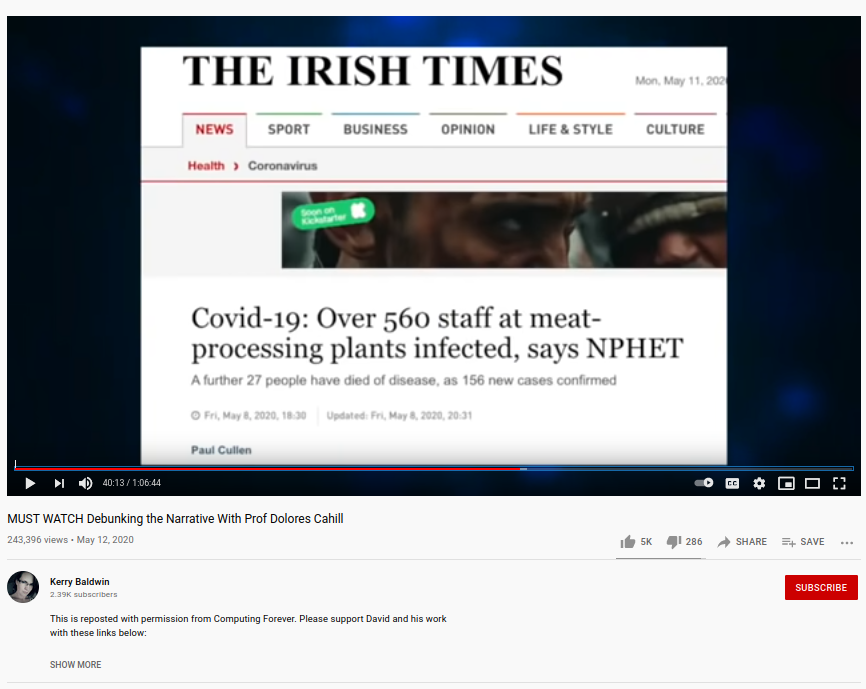
\includegraphics[scale=0.2]{./img/youtube_panels/news_without_banner.png} 
	\caption{Screenshots showing two duplicates of the same video, taken on July 21, 2021. 
Left panel: a \href{https://www.youtube.com/watch?v=d9GbVZOcT18}{YouTube video} about COVID-19 without an information panel. 	
Right panel: a \href{https://www.youtube.com/watch?v=A4RvrEKoNxc}{duplicate of the same video} uploaded under a different title and with a `COVID-19 vaccine' information panel.}
	\label{duplicates_yt}
\end{figure}



%\subsection{Blocking links}

%\subsubsection{Twitter}

%\href{https://help.twitter.com/en/safety-and-security/phishing-spam-and-malware-links}{link}


\section{Reducing the visibility}

Mainstream social media platforms can reduce the visibility of content created or shared by users, whenever they violate the platforms' rules. 
The implementation of this policy varies across platforms and is not easy to verify ex-post. In what follows we provide indirect methods to explore how reducing the visibility of content works on Facebook, Twitter and YouTube. 
 

\subsection{Facebook} \label{reduce_fb}


To tackle misinformation, Facebook can reduce the spread of misleading content through their built-in ranking system. 
More specifically, Facebook ranks each post and/or ad by assigning to it a relevancy score, where a high score leads to a high likelihood of the post and/or the ad to appear on a user's newsfeed. Doing so, Facebook can make a post or a whole account less visible by decreasing the relevancy score of its content; this is precisely the $reduce$ measure (see the article on Facebook Newsroom (2018)~\cite{newsroom2}). This measure can be verified by looking at the number of views (reach) of a post, but this metric is not available via the APIs used to access Facebook data: CrowdTangle or BuzzSumo. Hence we can indirectly investigate the $reduce$ measure by looking at the engagement metrics (likes, comments, shares) related to a given post; which are available on CrowdTangle and BuzzSumo. If a post reaches less users because it has a lower ranking, then it is less likely to receive likes, comments and shares, relative to a post with a higher ranking. 

% Owned by Alex Jones, Infowars is usually described as a misinformation website: it is on the Wikimedia global spam blacklist\footnote{See \href{https://meta.wikimedia.org/wiki/Spam\_blacklist}{meta.wikimedia.org/wiki/Spam\_blacklist}.},
%CrowdTangle and Buzzsumo provide access to the interaction metrics on content (engagement), but not to the number of views (or reach), therefore we can only verify the {\it reduce} measure indirectly through a decrease in engagement. If Facebook was reducing the reach of a content via a lower ranking, we would expect the content to be less likely to receive likes, comments and shares, relative to a post with a higher ranking.

\smallskip

To illustrate, we investigate the case of the website $Infowars$. This website appears in the Misinformation Directory of FactCheck.org, among other websites who have posted deceptive content\footnote{See \href{https://www.factcheck.org/2017/07/websites-post-fake-satirical-stories/}{https://www.factcheck.org/2017/07/websites-post-fake-satirical-stories/}.}. Furthermore, the factual reporting of $Infowars$ has been rated {\it very low} by the Media Bias / Fact Check resource of Iffy.news and it has several failed fact-checks reported by Feedback.org.\footnote{See the Iffy.news page \href{https://mediabiasfactcheck.com/infowars-alex-jones/}{https://mediabiasfactcheck.com/infowars-alex-jones/} and Feedback.org \href{https://open.feedback.org/media/RM}{https://open.feedback.org/media/RM}.} 

On May 2, 2019, Facebook announced they would prohibit users from sharing Infowars content unless, they are explicitly condemning the material.\footnote{See the article in Wired by Martineau (2020)~\cite{wiredalexjones} and see the section {\it So what happened with InfoWars? They were up on Friday and now they are down?} \href{https://about.fb.com/news/2018/08/enforcing-our-community-standards/}{about.fb.com/news/2018/08/enforcing-our-community-standards/}.} To verify the measure, we used the ``/posts/search'' endpoint\footnote{see the documentation for more details: \href{https://github.com/CrowdTangle/API/wiki/Search}{github.com/CrowdTangle/API/wiki/Search}.} of the CrowdTangle API, to collect $37$ $242$ Facebook public posts that had shared a URL link containing ``infowars.com'', published between January $1$, $2019$ and December $31$, $2020$.\footnote{We found in the collected data some Facebook posts that did not directly share an Infowars link (but rather a YouTube or Facebook video containing an Infowars link in its description), thus we excluded such posts from our data to keep only the $27$ $721$ posts directly sharing an Infowars link.} 

\begin{figure}[h]
\hspace{-2em}
	%\centering
		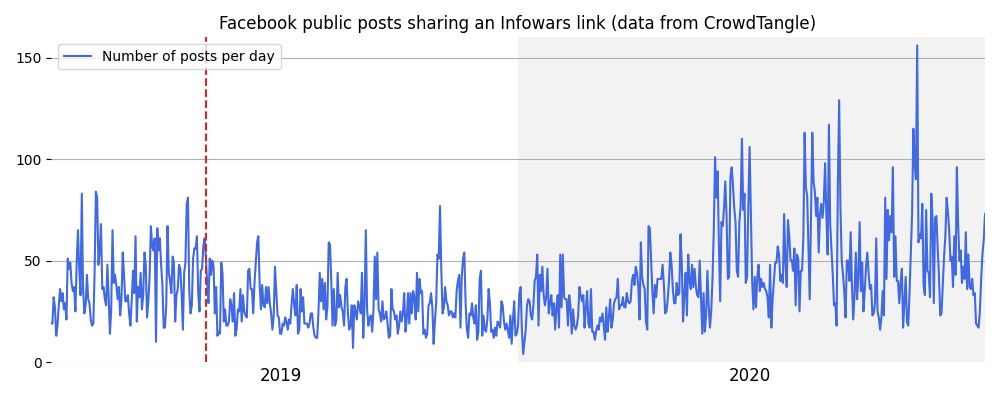
\includegraphics[scale=0.32]{../figure/facebook_crowdtangle_infowars_1.png}
		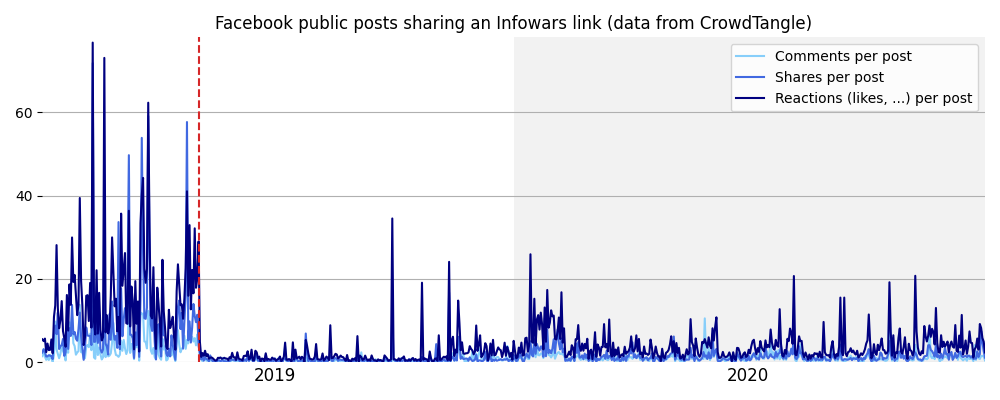
\includegraphics[scale=0.32]{../figure/facebook_crowdtangle_infowars_2.png} 
	\caption{Public Facebook posts sharing an Infowars link in $2019$ and $2020$ collected from the CrowdTangle API. The red line marks the date of May $2$, 2019, when Facebook has announced the ban regarding Infowars. (Top panel) Number of daily posts. (Bottom panel) Engagement metrics: average number of reactions, shares and comments per post. }
	\label{infowars1}
\end{figure}

The number of public posts sharing an $Infowars$ link remained globally stable throughout $2019$ (see figure \ref{infowars1} left panel). 
Thus the measure announced by Facebook does not seem to have prevented users from sharing an $Infowars$ link. Nevertheless, a clear drop in engagement was observed on May $2$, $2019$ (see figure \ref{infowars1} right panel). 
The number of reactions, shares and comments per post have decreased respectively  by $-94\%$,  $-96\%$ and $-93\%$  when comparing the two months before and after May $2$, $2019$. This suggests the measure taken by Facebook in May $2019$, is not a ban per se, but rather a $reduce$ measure. This is because users could still post $Infowars$ links, but these posts generated less engagement. It should be noted that the engagement metrics increased again by the end of $2019$ / beginning of $2020$, suggesting that the $reduce$ measure may have been lifted a few months after its implementation.

Another measure that platforms can apply is to prevent users from sharing specific types of content, like URLs belonging to a specific domain name.  
The Beauty of life (\href{https://thebl.com/}{thebl.com/}) is a US-based media company that shares pro-Trump views and conspiracy theories such as QAnon.
\footnote{ See \href{https://en.wikipedia.org/wiki/The\_Epoch\_Times\#Removal\_of\_The\_BL\_(The\_Beauty\_of\_Life)\_from\_Facebook}{wikipedia article}.} 
Facebook has announced on December $20$, $2019$ that ``The BL is now banned from Facebook''.
\footnote{\url{https://about.fb.com/news/2019/12/removing-coordinated-inauthentic-behavior-from-georgia-vietnam-and-the-us/}}

To verify Facebook’s ban, we first tested whether we could post a Facebook message containing a url from thebl.com. This turned out to be impossible. But such manual verification cannot inform us whether the ban applies indeed to all Facebook users and accounts (as we used only our own personal accounts), nor when it has started. To further investigate this policy, we collected data from the BuzzSumo API\footnote{BuzzSumo is a commercial content database that tracks the volume of user interactions with internet content on Facebook, Twitter, and other social media platforms.}. We used the ``/search/articles'' endpoint to collect the engagement metrics of the $13$ $634$ articles crawled from the $thebl.com$ website between January $1$, $2019$ and June $15$, $2021$.

\begin{figure}[h]
\hspace{-2em}
	%\centering
		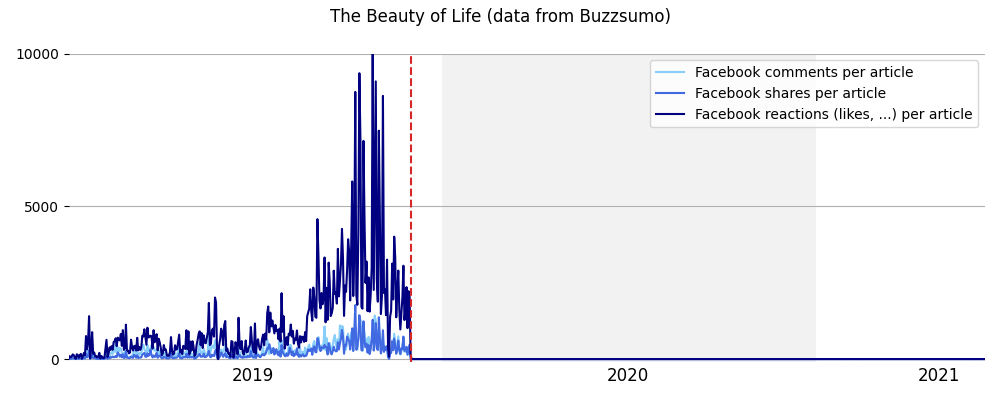
\includegraphics[scale=0.32]{../figure/facebook_buzzsumo_thebl_1.png}
		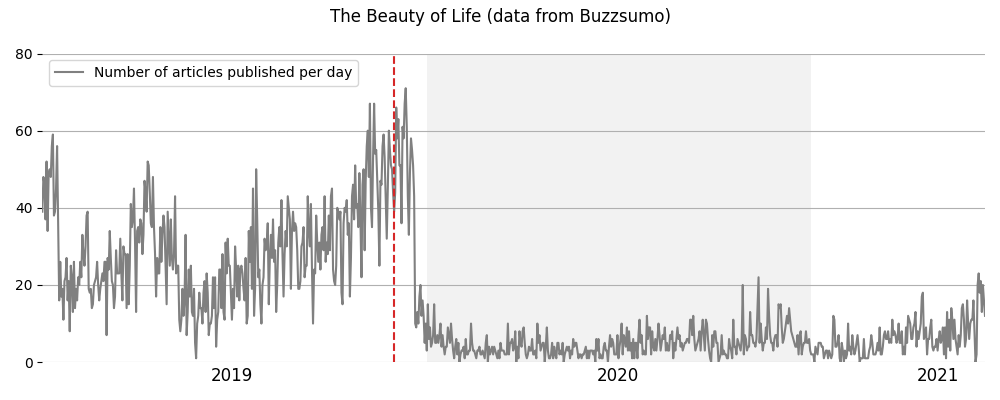
\includegraphics[scale=0.32]{../figure/facebook_buzzsumo_thebl_2.png} 
	\caption{Articles from The Beauty of Life website (thebl.com) published between January 1, 2019 and June 15, 2021 and gathered from the Buzzsumo API. Left panel: Facebook engagement metrics (average number of reactions, shares and comments per article). Right panel: Number of articles published per day. The red line marks the date of December 1, 2019. }
	\label{fb_bl}
\end{figure}

The number of Facebook reactions, shares and comments dropped to zero for TheBL’s articles published after December $1$, $2019$ (see figure \ref{fb_bl} top panel), indicating the start of the ban. We can note that although the ban was communicated in an article published on December $20$, $2019$, it seems to have actually started on December $1$, $2019$. The communication around the ban appeared to have discouraged The Beauty of Life to proceed with their activity. Indeed the number of articles they published daily was around $50$ until December $20$, $2019$, when it decreased drastically to reach around $5$ to $10$ articles published per day (see figure \ref{fb_bl} bottom panel). 

Using BuzzSumo data, we ascertained that links from thebl.com were not shared on Facebook anymore. The ban started on December $1$, $2019$, and appeared to be still enforced in June 2021.

\subsection{Twitter}  \label{globalresearch}

Twitter can take action against a tweet which violates the Twitter rules, by limiting its visibility\footnote{See the paragraph {\it Limiting Tweet visibility}: \href{https://help.twitter.com/en/rules-and-policies/enforcement-options}{https://help.twitter.com/en/rules-and-policies/enforcement-options}.} on users' timelines and in search results. To illustrate we provide an example for the website $globalresearch.ca$, which has several failed fact-checks according to \href{https://open.feedback.org/media/AEKA}{Feedback.org} and \href{https://iffy.news}{iffy.news} - two websites which provide databases of websites with low factual reporting levels.\footnote{For $globalresearch.ca$ see \href{https://open.feedback.org/media/AEKA}{open.feedback.org/media/AEKA} and \href{https://mediabiasfactcheck.com/global-research/}{https://mediabiasfactcheck.com/global-research/}.}

\begin{figure}[h]
	\centering
%\hspace{-2em}
	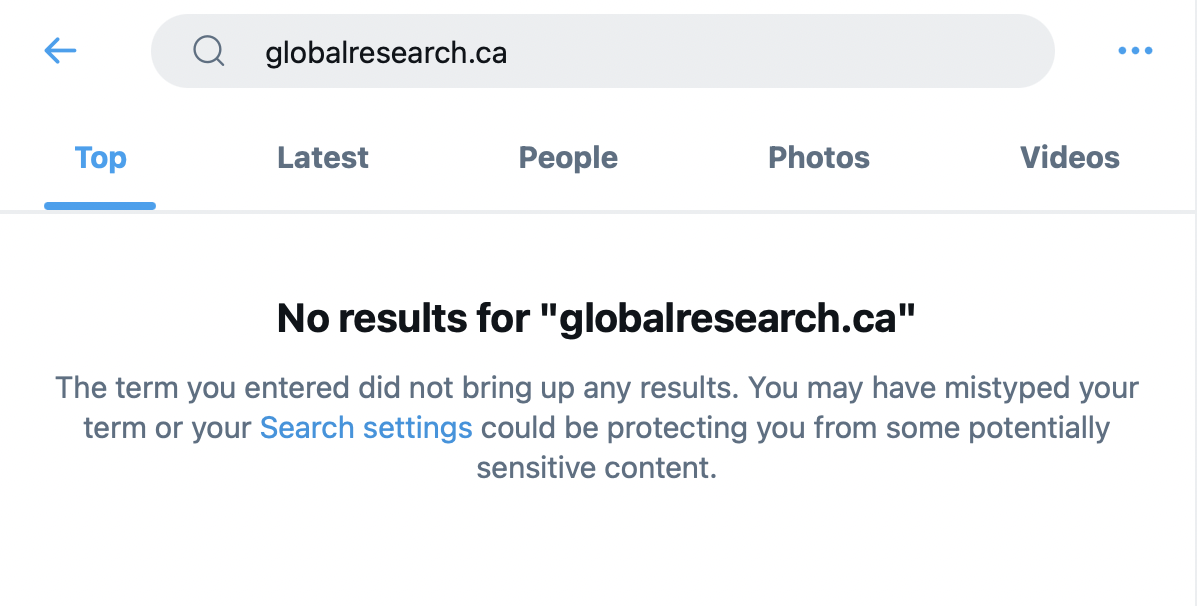
\includegraphics[scale=0.32]{./img/globalresearch_14_06_2021_16pm_UTC.png} 
	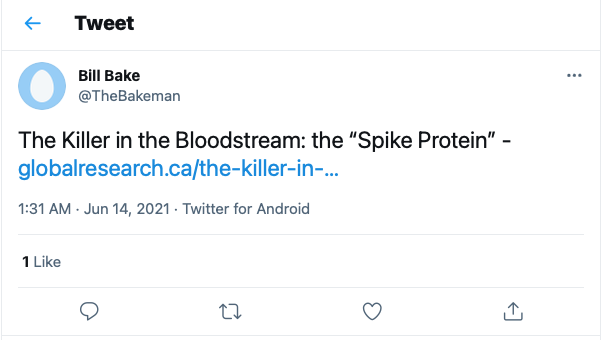
\includegraphics[scale=0.32]{./img/globalresearch/tweet.png} 

	\caption{Screenshots taken on June 14, 2021. Left Panel: screenshot that shows that no results can be found when searching for articles linked to the domain name $globalresearch.ca$ via the Twitter search box. Right Panel: example of a tweet posted on June $14$ containing the domain name {\it globalresearch.ca}. }
		\label{fig3}
\end{figure}

\smallskip

When a user searches via the twitter search-box for this domain name, no results appear as shown in the screenshot in the left panel of figure \ref{fig3}, taken on June $14$, $2021$. To further investigate the possible implementation of a reduced visibility measure, we searched via the Twitter API v2 for tweets, excluding retweets, containing the query {\it globalresearch.ca} from April $15$, $2021$ until August $15$, $2021$.  As shown in the left panel in figure \ref{fig4}, we find a strictly positive number of tweets containing the domain name {\it globalresearch.ca} after the date on which the screenshot was taken (left panel of figure \ref{fig3}). Hence, the visibility of tweets containing this domain name has been reduced because users can no longer access tweets containing the domain name {\it globalresearch.ca} via the search box. Nevertheless users are not restrained from posting tweets containing this domain name, as shown in the screenshot in panel $(b)$ of figure \ref{fig3}, found by taking the tweet ID of one of the collected tweets via the Twitter API. Furthermore, those collected Tweets have strictly positive engagement metrics as shown in panel $(b)$ of figure \ref{fig4}. Hence, the users who post tweets including articles from the {\it globalresearch.ca} website receive tweet level engagement from their own followers. 

\begin{figure}[h]
%\centering
\hspace{-2em}
		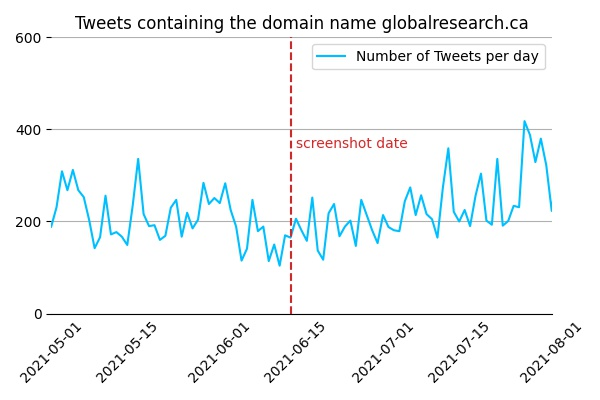
\includegraphics[scale=0.32]{../figure/globalresearch_domain_2021-08-17.jpg} 
		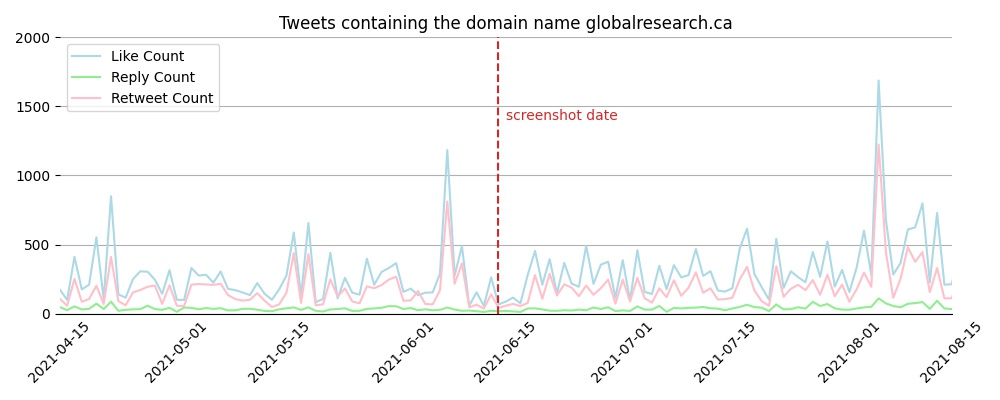
\includegraphics[scale=0.32]{../figure/globalresearch_domain_engagement_2021-08-17.jpg}
\caption{Left Panel: daily number of Tweets, excluding retweets, containing the query {\it globalresearch.ca} from January $1$, $2021$ until June $30$, $2021$. Right Panel: engagement metrics of Tweets containing the query {\it globalresearch.ca} from January $1$, $2021$ until June $30$, $2021$. Data collected via the Twitter API v2 on August $17$, 2021.   }
\label{fig4}
\end{figure}

Finally, the website $globalresearch.ca$ is linked to the Twitter account {$@CRG\_CRM$} and it was recently suspended from Twitter. We noticed the message about the account suspension (see the right panel in figure \ref{fig4bis}) on May $25$, 2021. To the best of our knowledge, no official communication by Twitter has announced the suspension nor the exact date at which it was implemented. Hence the account may have gotten suspended before that date. Furthermore when a user attempts to click on a link which contains {\it globalresearch.ca} in a Tweet, a warning message appears and indicates that the link may be unsafe (see the left panel in figure \ref{fig4bis}). For the case of this Twitter account, it is likely that a mix of interventions was used: reducing the visibility via the search box, suspending the related Twitter account and returning a warning message when users click on a link containing this domain name.  


\begin{figure}[h]
	\begin{center}
	\resizebox{.9\textwidth}{!}{%
		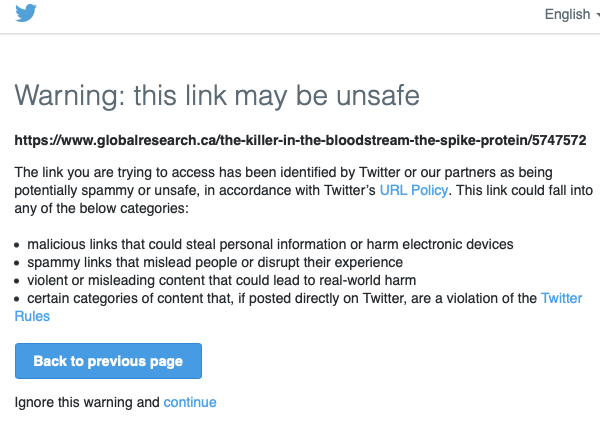
\includegraphics[height=3cm]{./img/globalresearch/warning.png} 
		\quad
		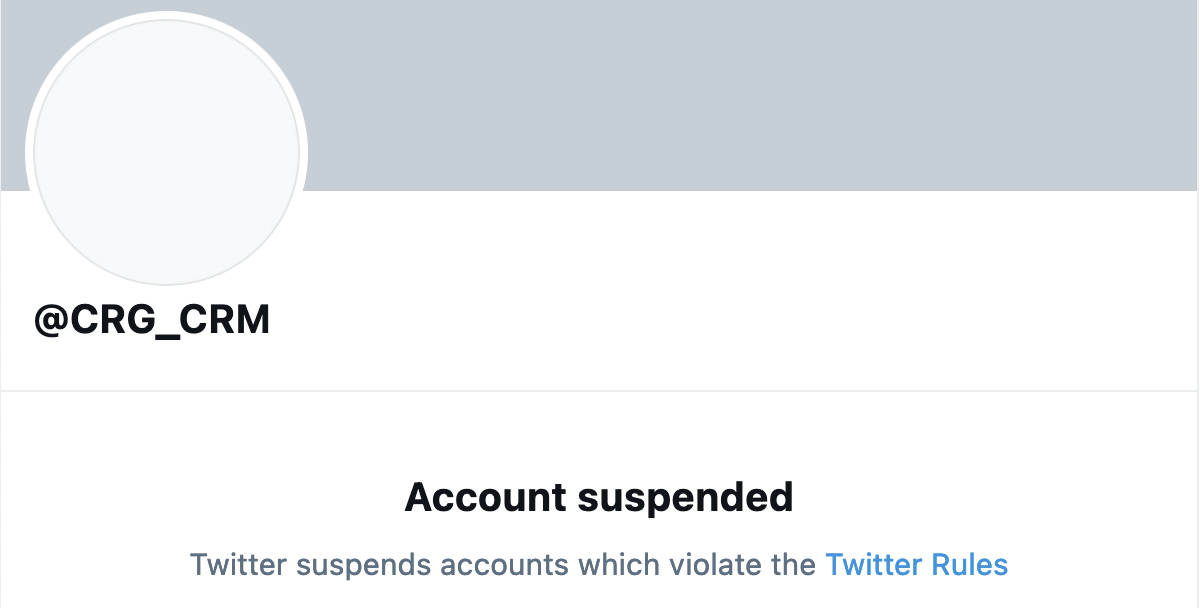
\includegraphics[height=3cm]{./img/globalresearch/globalresearch_2021-06-14.png}
	}
	\end{center}
	\caption{Screenshots taken on June 14, 2021. Left Panel: warning message that appears when a user attempts to click on a link which contains the domain name {\it globalresearch.ca}. Right Panel: account suspension message of $@CRG$\_$CRM$ linked to {\it globalresearch.ca}.  }
	\label{fig4bis}
\end{figure}

%We provide a second example with the website $off$-$guardian.org$. Unlike the previous example, the Twitter account linked to this website is not currently\footnote{The account can be accessed via the Twitter handle $@OffGuardian0$ and we verified on June 13, 2021 that the account is not suspended.} suspended. 

%off guardian: people put space before .com but they can still share off-guardian links  (test Héloïse). why do they do that? 
%warning page before accessing the website - always 
%twitter API doesn't return the tweets tweeted by off-guardian themselves dating back to 2015
%twitter API returns both tweets with . org and .org: 320 tweets from 2017-01-15 until 2021-06-11. But off-guardian themselves posted one of their own links on June 16 2021. 
%minet returns almost nothing : 43 tweets 
% the tweets created by Off-Guardian: don't come up in the search box. Unlike nytimes.com their articles do appear in the search box , published by themselves! 
% Heloise's tweet June 15 doesn't come up in the API ! 
% people use variants with * and dot , so that they can find tweets speaking about those domains

\subsection{YouTube}

YouTube can reduce the visibility of some video content via its recommendation system, namely by recommending content from authoritative sources for topics related to science and health. This platform recommends content to the users based on the watch history and searched queries in google and YouTube; which can both be cleared via account settings. Moreover, a recommendation system based on preferences and history might have a down side, namely when a user repeatedly watches videos that might be misleading or that promote conspiracy theories. YouTube states that they set out to prevent their systems from serving up content that could misinform users in a harmful way, particularly in domains that rely on veracity, such as science, medicine, News, or historical events.  YouTube identifies misinformation by using external human evaluators and experts to examine if a given video is promoting misleading information or conspiracy theories. Then using the feedback of the evaluators, they use machine learning systems to develop models that generate recommendations. The models work on reviewing videos daily to reduce the spread of misinformation. 

\smallskip

To examine this effect, we designed an experiment that simulates a user's behavior on YouTube. We used a list of $45$ videos marked as {\it False} by Science Feedback and classified under the category ``health'' (see section \ref{youtube_panels} for the classification). The experiment starts with one video marked as ``False'' from our list of videos and a clean watch history. For each video, our automated program collects around\footnote{Notice that as we are simulating the behavior of a user, when we visit a video, we get a number of recommendations that vary between $18$ videos and $22$ videos.} $20$ recommendations and clicks on the top $10$ videos in sequential order. After that, for every video in the set of the top $10$ recommendations, we collect their top $20$ recommended videos. In addition, to simulate a user's behavior, the automated program watches each video for a few minutes\footnote{If the video duration is ten minutes or less, the automated program watches the whole video. If the video duration is strictly higher than ten minutes, then the automated program watches only five minutes.}. Doing so, we collected $10$ $549$ YouTube recommended video entries, among which only $3$ $895$ were unique. 
To analyse the collected data, we look for misinformation: $(i)$ at the video level and $(ii)$ at the channel level. 

\smallskip

{\bf Video Level.} We ranked the recommended videos based on the number of times they got recommended. We then asked Science Feedback to fact-check the top 40 recommended videos.
Those $40$ videos were recommended $1$ $735$ times out of the $10$ $549$ YouTube recommended video entries (that is $16\%$ of the recommendations).
Among the top 40 recommended videos, four unique videos were marked as {\it misleading} and they were recommended $132$ times out of the $1$ $735$ recommendations (that is $7.7\%$ of the recommendations).
Four other videos were marked as {\it hyper-partisan} and they were recommended $184$ times ($10.7\%$).

\smallskip 

\begin{figure}[h]
	\begin{center}
		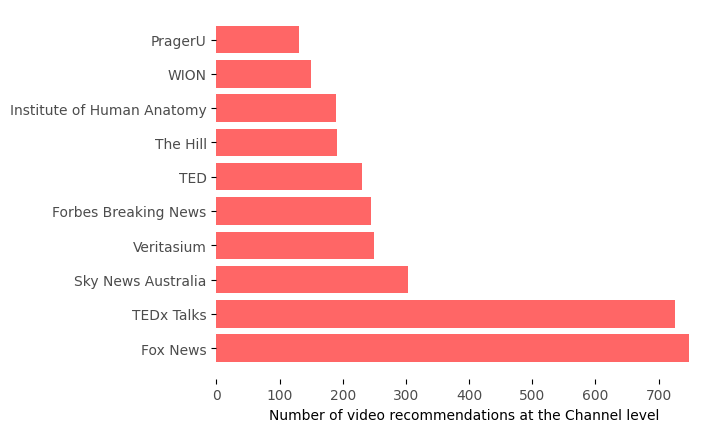
\includegraphics[scale=0.45]{./img/channel_youtube.png} 
	\end{center}
	\caption{Top ten recommended channels among the $1$ $562$ different channels, that have posted the recommended videos in our dataset.}
	\label{channels_yt}
\end{figure}

{\bf Channel Level.} We examined the top recommended channels in the collected data. We got $1$ $562$ different channels, and we counted the number of times every channel got recommended. Figure \ref{channels_yt} shows the top $10$ recommended channels, whose videos represent $30\%$ of the total set of recommended videos in our dataset. Among the top three most recommended channels, there is Fox News and Sky News Australia, which both have a ``mixed'' factual reporting level according to {\it iffy.news} and have several failed fact-checks.\footnote{See \href{https://mediabiasfactcheck.com/fox-news-bias/}{https://mediabiasfactcheck.com/fox-news-bias/} and \href{https://mediabiasfactcheck.com/sky-news-australia/}{https://mediabiasfactcheck.com/sky-news-australia/}.} Also in the top ten most recommended, we find PragerU, which has a ``low'' level of factual reporting according to {\it iffy.news}. 

\smallskip 

At the video level, we start at each round with a YouTube video marked as ``False'' and we expected to have a high proportion of misinformation videos. But only {$18.4\%$} of the recommendations corresponded to $misleading$ or {\it hyper-partisan} videos.
This relatively small percentage hints towards that idea that YouTube is probably reducing the visibility of videos containing misinformation. However, when we investigated misinformation at the channel level, we found that videos belonging to channels that are not highly authoritative were being often recommended. In other words, it is likely that YouTube acts on reducing the visibility of videos but not channels, via its recommendation system. Notice that the policy of reducing the visibility of misleading content is hard to prove on YouTube in general, given the complexity of their recommendation algorithm.

\section{Discussion}

In this article we have assessed three broad categories of interventions to tackle misinformation by Facebook, Twitter and YouTube: $(i)$ suspension of accounts, $(ii)$ introduction of flags, labels and information panels and $(iii)$ reducing the visibility of content.\footnote{For a detailed list of interventions of multiple platforms, we invite the reader to navigate through the following \href{https://airtable.com/shrO0ooI9WSEfIUhb/tblAWQwFOiihKdQjm/viwZLAOzLK1NQ0c2n?blocks=hide}{airtable} compiled by Slatz and Leibowicz (2021)~\cite{niemanlab}.}
Furthermore, we have provided a methodology that can be useful for third-party monitoring. 
The code needed to collect the data and create the figures is available on the following public GitHub repository: \href{https://github.com/medialab/truth-and-trust-online-2021/}{https://github.com/medialab/truth-and-trust-online-2021/}, and we hope it can be a useful ressource for researchers, NGOs and journalists addressing online misinformation. 

\smallskip

Mainstream platforms such as Facebook, Twitter and Youtube are increasingly working towards higher data transparency (see links that redirect to the respective transparency centers in Appendix \ref{links}). 
Yet the present research sheds light on the restrictions to access data and its limits, which impede the academic community from studying successfully online misinformation and assessing the impact of platforms' interventions regarding this phenomenon. 
Hence, few comments are in order regarding the limitations to access data, the lack of transparency vis-\`{a}-vis misinformation related interventions and the lack of interventions designed specifically for misinformation. 

\smallskip

{\bf A need for more complete data.} 
When Facebook, Twitter or YouTube intervene by suspending an account, the data can no longer be accessed via scraping or via the official APIs (Twitter, YouTube, CrowdTangle) for the purposes of scientific research. 
This hampers the investigation of how platforms moderate content. 
To further illustrate this point, the original list of YouTube videos with failed fact-checks (summarized in Table \ref{tab2}), had over $200$ YouTube videos available in March $2021$. 
However, by June $2021$, thirty videos had disappeared from the YouTube API for policy violation. 
Similarly, in a related research project (see Thero and Vincent (2020)~\cite{therovincent}) we searched on CrowdTangle for $94$ public accounts sharing specific content associated with misinformation in November $2020$. 
We tried to collect the posts from those $94$ pages in January $2021$, to only discover that $11$ pages had disappeared from the CrowdTangle API.
It is of course not surprising that platforms are regulating their content, sometimes by removing it. 
Nevertheless, researchers' work could be simplified, if deleted data could still be accessible via the APIs.

Although it is currently impossible to verify permanent deletions using available social media data, their effects can be observed using an adapted methodology.
Following the Capitol riots in January $2021$, Twitter has announced the suspension of more than $70$ $000$ accounts related to QAnon.\footnote{\href{https://blog.twitter.com/en\_us/topics/company/2021/protecting--the-conversation-following-the-riots-in-washington--}{https://blog.twitter.com/en\_us/topics/company/2021/protecting--the-conversation-following-the-riots-in-washington--}.} 
A journalist has recently investigated the effects of this measure by counting the number of times hashtags related to the QAnon movement have been used over time, such as \#QAnon or \#WWG1WGA.
A drastic reduction in hashtag use was found when comparing the first quarter of $2021$ with the first quarter of $2021$.\footnote{See \href{https://twitter.com/Shayan86/status/1394742784683298818}{https://twitter.com/Shayan86/status/1394742784683298818}.}
Thus, counting specific hashtag use over time allows to indirectly observe permanent suspensions on Twitter and there is a need for similar methodologies to be experimented on data from other platforms.
However, a point of concern is that data can also disappear because of other factors independent of platforms' content moderation.
To provide an example, McMinn et al. (2012)\cite{mcminn2013building} collected $120$ million tweets related to general topics. 
The same published set of Tweet IDs was then used by Mazoyer et al. (2020)~\cite{mazoyer2020french}, to run the same collection in $2018$. Mazoyer et al. 2020~\cite{mazoyer2020french} were only able to retrieve $67$ millions of tweets (55\%). The authors argue that this drop is probably due to tweets having been removed by users and Twitter accounts being shut by the users themselves.
As data can disappear from platforms over time, it is hard to distinguish whether platforms or users are the ones responsible for data removal. 
Hence in the special case of Twitter accounts related to QAnon, it is hard to identify how much of the drop in QAnon related hashtag use is due to the Twitter intervention or to accounts migrating to other platforms out of fear of having their accounts suspended by the platform.

\smallskip 

Aside from the disappearance of data due to content moderation, some essential metrics for the study of misinformation are not accessible via main APIs. 
In particular, the $reach$ of posts on Facebook, which is the number of people who actually see a given post, cannot be recovered from the CrowdTangle API.
\footnote{See \href{https://help.crowdtangle.com/en/articles/4558716-understanding-and-citing-crowdtangle-data}{https://help.crowdtangle.com/en/articles/4558716-understanding-and-citing-crowdtangle-data}.} 
Hence, researchers can only build proxies for this metric based on available data (see section \ref{reduce_fb} for an example). 
Furthermore, to the best of our knowledge, fields related to flags, notices and information panels are not available on the official APIs, with the exception of the {\it withheld}  and {\it possibly sensitive content} interstitials in the Twitter API v2. 
For the purposes of the present research we thus had to scrape this information from publicly available content on Facebook, Twitter and YouTube. 
Again, this disrupts the monitoring of the platforms' interventions and the assessment of their impact (Pasquetto, Swire-Thompson, Amazeen et al. (2020)~\cite{pasquetto}).

\smallskip

A last concern regards the growing restrictions to access APIs (Perriam et al.(2019)~\cite{api}).
In April $2018$, likely as a response to the Cambridge Analytica scandal, Facebook severely limited access to their official APIs\footnote{See \href{https://about.fb.com/news/2018/04/restricting-data-access/}{https://about.fb.com/news/2018/04/restricting-data-access/} and \href{http://thepoliticsofsystems.net/2018/08/facebooks-app-review-and-how-independent-research-just-got-a-lot-harder/}{http://thepoliticsofsystems.net/2018/08/} \href{http://thepoliticsofsystems.net/2018/08/facebooks-app-review-and-how-independent-research-just-got-a-lot-harder/}{/facebooks-app-review-and-how-independent-research-just-got-a-lot-harder/}.} 
and CrowdTangle is today a reliable source for researchers to access Facebook data. 
However, it should be noted that CrowdTangle has been recently used by journalists to show that Facebook is spreading biased information\footnote{See the news article \href{https://www.economist.com/graphic-detail/2020/09/10/facebook-offers-a-distorted-view-of-american-news}{https://www.economist.com/graphic-detail/2020/09/10/facebook-offers-a-distorted-view-of-american-news} and the tweet \href{https://twitter.com/facebookstop10}{https://twitter.com/facebookstop10}. 
The last link is a Twitter account showing each day the ten most shared link on Facebook, most of them coming from extreme right and misinformation sources. 
Facebook has reacted to this here: \href{https://about.fb.com/news/2020/11/what-do-people-actually-see-on-facebook-in-the-us/}{https://about.fb.com/news/2020/11/what-do-people-actually-see-on-facebook-in-the-us/}.} 
and a general suspicion is growing that its access might be shut down in a near future to journalists and researchers.\footnote{See the news articles \href{https://www.nytimes.com/2021/07/14/technology/facebook-data.html}{https://www.nytimes.com/2021/07/14/technology/facebook-data.html} and \href{https://www.bloomberg.com/news/articles/2021-08-03/facebook-disables-accounts-tied-to-nyu-research-project}{https://www.bloomberg.com/news/articles/2021-08-03/facebook-disables-accounts-tied-to-nyu-research-project}.}
Regarding Twitter and YouTube, it is still possible and relatively easy to access their official APIs. Nevertheless the number of Tweets that can be retrieved has decreased between the Twitter API v1 and v2. 
In the v2, there is a monthly cap of $10,000,000$ Tweets for the academic research track\footnote{https://developer.twitter.com/en/docs/projects/overview},
while in the v1 there was no monthly limit and only a limit on the number of requests that could be made in a 15-minute window\footnote{https://developer.twitter.com/en/docs/twitter-api/v1/rate-limits}.
We thus noticed that we could get around $10$ times more Tweets per month with the v1 when compared to the v2 for one specific collection.

\smallskip

{\bf A need for more transparency.} 
Mainstream platforms generally lack transparency regarding their misinformation related interventions.
The broad lines of policies regarding misinformation are communicated via blog posts and are not typically part of the set of rules or community guidelines of mainstream platforms (see Appendix \ref{links}).
Yet, when navigating through the categories of policy areas, to the best of our knowledge, misinformation is absent from the data available on the transparency centers of Facebook, Twitter and YouTube.
Platforms' official communication about misinformation interventions is scarce and the academic community, NGOs and data journalists, usually discover interventions related to misinformation via monitoring social media accounts related to domain names with several failed fact-checks or via articles in News outlets. 
For example, while conducting the present research, it was brought to our attention that the Twitter account related to the domain name $globalresearch.ca$ was suspended. 
But to the best of our knowledge, there was no official communication by the Twitter Safety team to explain the reasons of this suspension (see section \ref{globalresearch}). 

We are aware that full transparency regarding operational aspects of misinformation related interventions can backfire.
This is because the aimed users might find means to circumvent the interventions. 
We noticed that some YouTube channels are trying to avoid the likely automated COVID-19 information panels, by using notational variants such as ``C.O.V.I.D'' or ``C O V I D''. 
Similarly, we came across notational variants on Twitter of the domain name {\it off-guardian.org}
\footnote{Here is an example of a failed fact-check of one of the articles of the website {\it off-guardian.org} : \href{https://www.politifact.com/factchecks/2020/jul/07/blog-posting/covid-19-tests-are-not-scientifically-meaningless/}{politifact.com/factchecks/2020/jul/07/blog-posting/covid-19-tests-are-not-scientifically-meaningless/}}
such as {\it off-guardian. org}, {\it off-guardian .org}, {\it off-guardian./org}, {\it off-guardian*org}.\footnote{For this case, we failed to understand precisely what kind of intervention Twitter users were circumventing, since they could share in a Tweet an article redirecting to the website {\it off-guardian.org} with the correct notation and only a warning message would appear when one clicks on it.}
Hence, a balance is needed between: $(i)$ fully transparent communication about misinformation related interventions so that the users can understand how the platforms are regulating their content, and $(ii)$ not explicitly giving too much information which would allow the policies to be bypassed.

\smallskip

In certain cases, the platform interventions were not motivated by content moderation to limit misinformation, but rather by other rule violations.
For example, the official reason for the suspension of Donald Trump's Twitter account was not misinformation\footnote{Although Donald Trump may have spread many misinformation during his governance, see for example: \href{http://allianceforscience.cornell.edu/blog/2020/10/what-drove-the-covid-misinformation-infodemic/}{http://allianceforscience.cornell.edu/blog/2020/10/what-drove-the-covid-misinformation-infodemic/}.}
but the violation of Twitter's Glorification of Violence Policy, with his last tweets encouraging the Capitol's riot.\footnote{See \href{https://blog.twitter.com/en\_us/topics/company/2020/suspension}{https://blog.twitter.com/en\_us/topics/company/2020/suspension}.}
Similarly, when Facebook removed four pages related to the InfoWars website, the cited reason was repeated violations of Community Standards: 
``While much of the discussion around Infowars has been related to false news, which is a serious issue that we are working to address [...], none of the violations that spurred today’s removals were related to this''.\footnote{See the article \href{https://about.fb.com/news/2018/08/enforcing-our-community-standards/}{https://about.fb.com/news/2018/08/enforcing-our-community-standards/}.}
Regarding The Beauty of Life website, its ban was officially due to coordinated inauthentic behavior,\footnote{See \href{https://about.fb.com/news/2019/12/removing-coordinated-inauthentic-behavior-from-georgia-vietnam-and-the-us/}{https://about.fb.com/news/2019/12/removing-coordinated-inauthentic-behavior-from-georgia-vietnam-and-the-us/}.} 
which includes using fake accounts that misrepresent one's identity or using methods to artificially boost the popularity of content. 
According to Facebook, coordinated inauthentic behavior is a distinct phenomenon from disinformation, as ``most of the content shared by coordinated manipulation campaigns isn’t probably false''.\footnote{See: \href{https://about.fb.com/news/2019/10/inauthentic-behavior-policy-update/}{https://about.fb.com/news/2019/10/inauthentic-behavior-policy-update/}.} 
Nevertheless, both misinformation and coordinated inauthentic behavior were attested for the Beauty of Life, and reported to Facebook by the fact-checking organization Snopes.\footnote{See \href{ https://www.snopes.com/news/2019/11/12/bl-fake-profiles/}{https://www.snopes.com/news/2019/11/12/bl-fake-profiles/}, 
\href{https://www.snopes.com/news/2019/11/12/bl-fake-profiles/}{https://www.snopes.com/news/2019/11/12/bl-} \href{https://www.snopes.com/news/2019/11/12/bl-fake-profiles/}{fake-profiles/}  and 
\href{https://www.snopes.com/news/2019/12/13/facebook-bl-cib/}{https://www.snopes.com/news/2019/12/13/facebook-bl-cib/}.} 
In the above ``known'' examples, the compagnies' communication was very clear on the reason of the interventions (although one can suspect that the official reason given can depart from the real motivation behind an intervention). 
However, very often no official communication on behalf of the platforms can be found for a specific interventions observed in collected data. 
Because misinformation is often associated with creating fake accounts to speed its spread, and incitation to violence, it is sometimes unclear to distinguish between interventions due to misinformation and interventions due to other guideline violations, and more transparent communication on platforms' actions would help monitor the interventions specifically related to misinformation.

\smallskip

{\bf A need for more consistent and adapted policies.} Misinformation on the web is a problem that is increasingly discussed since the $2016$ American elections and in the years that followed, platforms may have decided on a case-by-case basis which actions to enforce.
Infowars and The Beauty of Life domains have both several failed fact-checks\footnote{They are both on the Iffy+ list, see \href{https://iffy.news/iffy-plus/}{https://iffy.news/iffy-plus/}.} and have both violated Facebook's community guidelines (incitation to violence and coordinated unauthentic behavior). 
Yet one's distribution was reduced for only half of a year, while the other one's links cannot be shared anymore on Facebook since the end of $2019$, and it is not clear why such double standard was applied on these comparable websites.
It is also possible that platforms usually follow specific rules on how to fight misinformation, but that sometimes the sudden media coverage of specific events leads them to take exceptional actions, such as with the Capitol riots and Trump's suspension from Facebook, Twitter and YouTube.
We would argue that to efficiently curb the spread of misinformation, policies should be clearly stated and consistently applied, rather than implementing interventions on a case-by-case basis and in response to the latest news events.

\smallskip

Furthermore, it is likely that most interventions used to tackle online misinformation correspond to interventions that were designed for earlier policy areas.
To illustrate, YouTube explicitly states
\footnote{See {\it What policies exist to fight misinformation on Youtube?} \href{https://www.youtube.com/intl/en\_us/howyoutubeworks/our-commitments/fighting-misinformation/\#policies}{youtube.com/intl/en\_us/howyoutubeworks/our-commitments/fighting-misinformation/\#policies}.}
that: ``Several policies in our Community Guidelines are directly applicable to misinformation'', such as the deceptive practices, impersonation and hate speech policies.
Hence interventions such as content deletion or account suspension, might be efficient for policy areas for which they were specifically designed, such as the policy area {\it Adult Nudity \& Sexual Activity}. Nevertheless, tackling online misinformation might need adapted interventions.
Namely, account suspensions or content deletion motivated by the spread of inaccurate information can be perceived as censorship by the targeted users. In particular, such interventions can generate platform migrations towards new alternative social media platforms (e.g. Telegram, Gab, Minds) with little or no content moderation (see Rogers (2020)~\cite{rogers2020}).

\smallskip

Finally, the means to tackle online misinformation is an active area of research and developing effective interventions against misinformation depends on understanding the psychology of interacting with social media (Pennycook and Rand (2021)~\cite{pennycook2021psychology}). 
Adding fact-checking labels to controversial content is certainly the intervention whose effectiveness was the most studied so far. 
It was shown that credibility indicators do reduce misperceptions and sharing, although their impact varied vastly depending on the presentation of the warnings (see Yaqub (2020)~\cite{yaqub2020effects} and Sharevski (2021)~\cite{sharevski2021misinformation}).
Moreover, a fact-checking label can lead to unpredicted consequences depending on the perception of the person reading it.
On Facebook, Twitter and YouTube, fact-checking messages are currently applied only to some content, while the rest of the content on a given platform remains naturally unlabelled. 
Such sparse application of warnings can lead to an ``implied truth'' effect, where users may assume that content without warnings have actually been verified and shown to be true (Pennycook et al. (2020)~\cite{pennycook2020implied}).
Using a different approach, Mosleh et al. (2021)~\cite{mosleh2021perverse} identified Twitter users sharing false news and replied to their false tweets with links redirecting to fact-checking websites.
They observed a decrease in the quality and accuracy of the content subsequently shared by the corrected user. 
These research papers highlight the necessity to investigate potential unintended effects of well-meaning interventions.
The methods presented in this paper can help to monitor not only the platforms' actions against misinformation, but also their subsequent consequences in real-life settings.

%\smallskip

% Recommendation to fight misinformation: inform about sources, example inform users that this account has shared x failed fact-checks over a x-months period.
	
% Networked public square / private companies / regulations / coordination... 

% User side: indirect effects, strategies... business model 

% Make point about how the three platforms communicate differently about their policies. 
%Need for a consistent policy for all, but this will surely come only when a law against misinformation is issued. 
%Facebook's strategy to tackle ``False News'' is three fold : Remove, Reduce, Inform. It is explained via a blog post on the facebook Newsroom. 
%Similarly, Twitter communicates about actions related to misinformation via their \href{https://blog.twitter.com/en\_us/authors.TwitterSafety}{Twitter Safety} Blog/account. 
%In a post on YouTube Official Blog, the platform explained its ``Four Rs of Responsibility" and how it raises authoritative content, reduces borderline content and harmful misinformation (see table \ref{summary} in Appendix \ref{links}).


\bibliography{proj1}{}
\bibliographystyle{plain}

\section{Appendix}

\subsection{Quick access to community guidelines and policies} \label{links}


\begin{landscape}

\thispagestyle{empty}

\begin{table}[p]
\centering
\setlength{\tabcolsep}{2pt}
\begin{tabular}{|c|c|c|}
\hline
\multirow{3}{*}{Rules}                     & 
\includegraphics[scale=0.05]{./img/fb_logo.png} & \begin{tabular}[c]{@{}cl@{}}   \href{https://www.facebook.com/communitystandards/recentupdates/}{facebook.com/communitystandards/recentupdates/}    \end{tabular}                     \\ \cline{2-3} 
                                           & 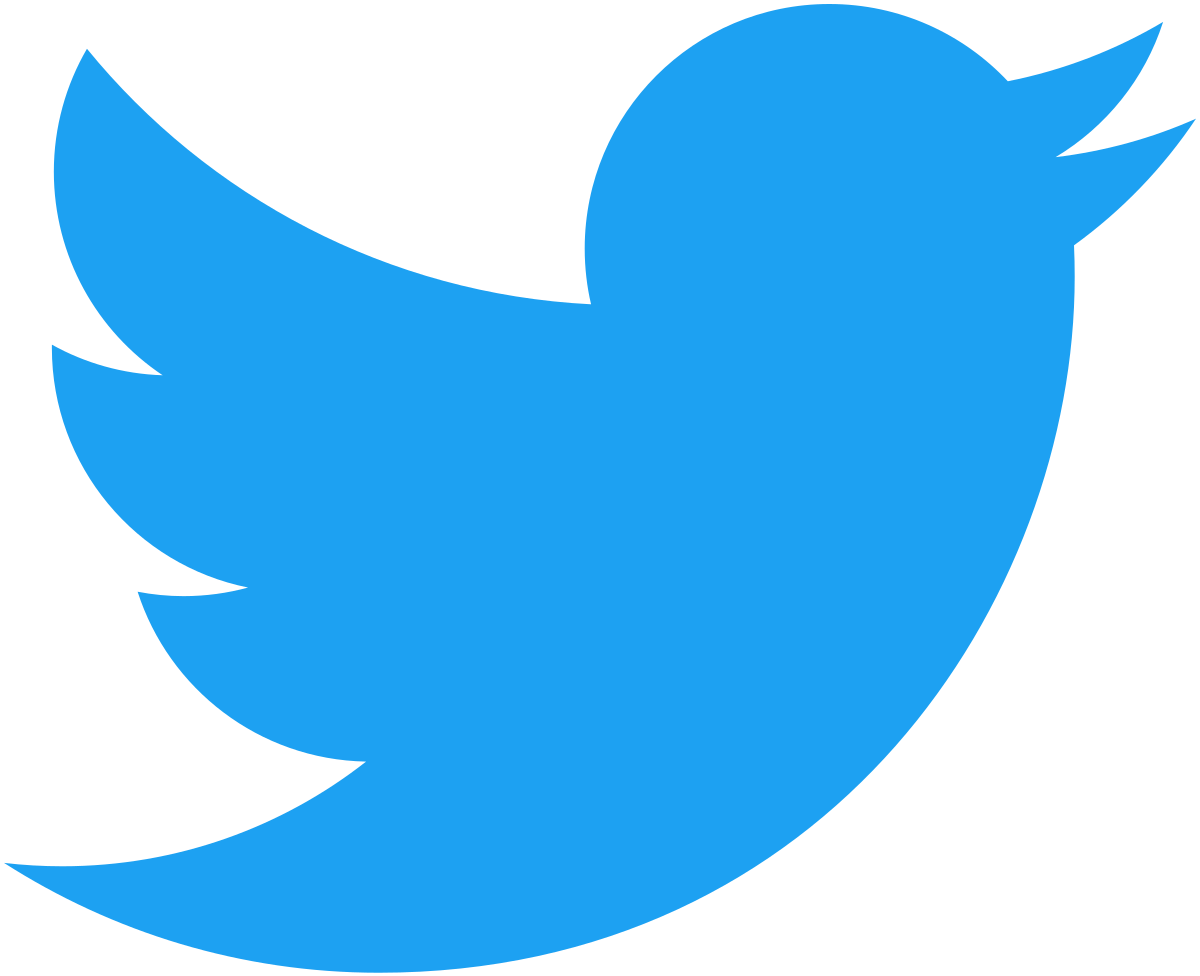
\includegraphics[scale=0.007]{./img/tw_logo.png}   & \href{https://help.twitter.com/en/rules-and-policies/twitter-rules}{help.twitter.com/en/rules-and-policies/twitter-rules}                       \\ \cline{2-3} 
                                           & 
\includegraphics[scale=0.03]{./img/yt_logo.png}  & \href{https://www.youtube.com/intl/en\_us/howyoutubeworks/policies/community-guidelines/}{youtube.com/intl/en\_us/howyoutubeworks/policies/community-guidelines/} \\ \hline
\multirow{3}{*}{\begin{tabular}[c]{@{}cl@{}}  Rules \\ enforcement \end{tabular}}         & 
\includegraphics[scale=0.05]{./img/fb_logo.png}  & \href{https://transparency.fb.com/data/community-standards-enforcement/}{transparency.fb.com/data/community-standards-enforcement/}                 \\ \cline{2-3} 
                                           & 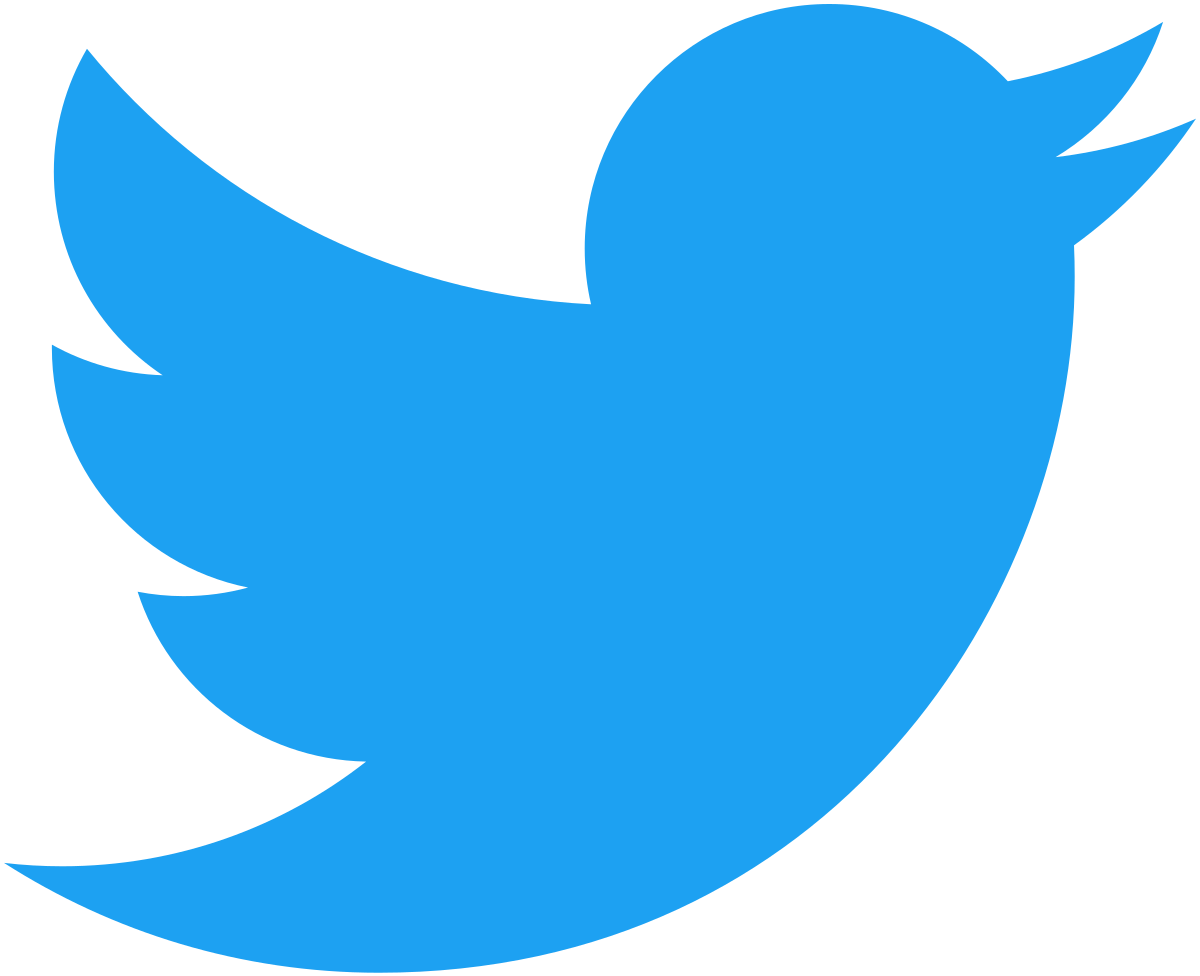
\includegraphics[scale=0.007]{./img/tw_logo.png}   & \href{https://transparency.twitter.com/en/reports/rules-enforcement.html}{transparency.twitter.com/en/reports/rules-enforcement.html}                \\ \cline{2-3} 
                                           & 
\includegraphics[scale=0.03]{./img/yt_logo.png}  & \href{https://transparencyreport.google.com/youtube-policy/}{transparencyreport.google.com/youtube-policy/}                              \\ \hline
\multirow{3}{*}{\begin{tabular}[c]{@{}cl@{}}  Transparency \\ center \end{tabular}}       & 
\includegraphics[scale=0.05]{./img/fb_logo.png} & \begin{tabular}[c]{@{}cl@{}}  \href{https://transparency.fb.com/data/}{transparency.fb.com/data/}    \\ \href{https://law.yale.edu/yls-today/news/facebook-data-transparency-advisory-group-releases-final-report}{https://law.yale.edu/yls-today/news/facebook-data-transparency-advisory-group-releases-final-report} \end{tabular}                                               \\ \cline{2-3} 
                                           & 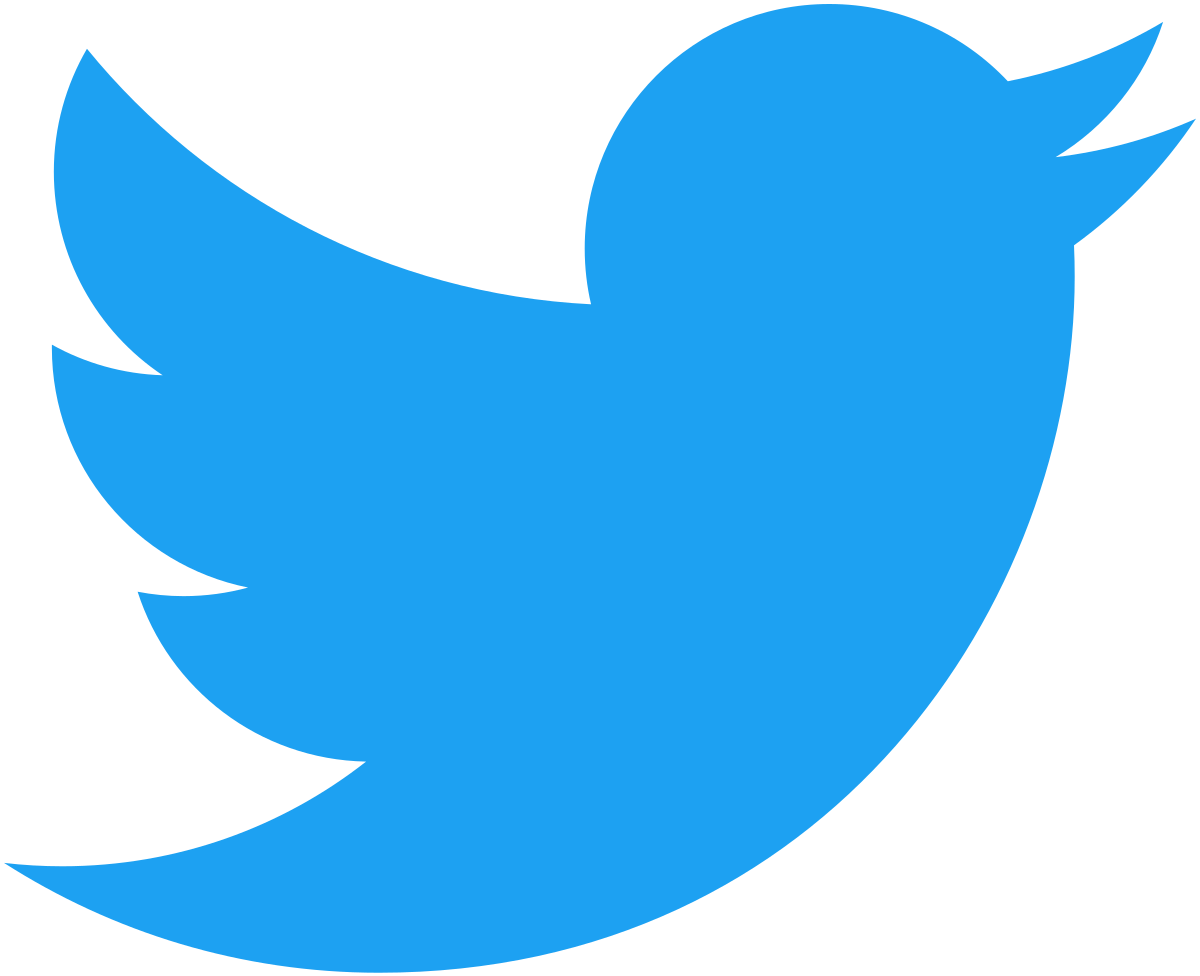
\includegraphics[scale=0.007]{./img/tw_logo.png}   & \href{https://transparency.twitter.com/en/reports.html}{transparency.twitter.com/en/reports.html}                                  \\ \cline{2-3} 
                                           & 
\includegraphics[scale=0.03]{./img/yt_logo.png}  & \href{https://transparencyreport.google.com/?hl=en}{transparencyreport.google.com/?hl=en}                                      \\ \hline
\multirow{3}{*}{\begin{tabular}[c]{@{}cl@{}}  Policy \\ regarding \\  Covid-19 \end{tabular}} & 
\includegraphics[scale=0.05]{./img/fb_logo.png} & https://www.facebook.com/help/230764881494641/                                     \\ \cline{2-3} 
                                           & 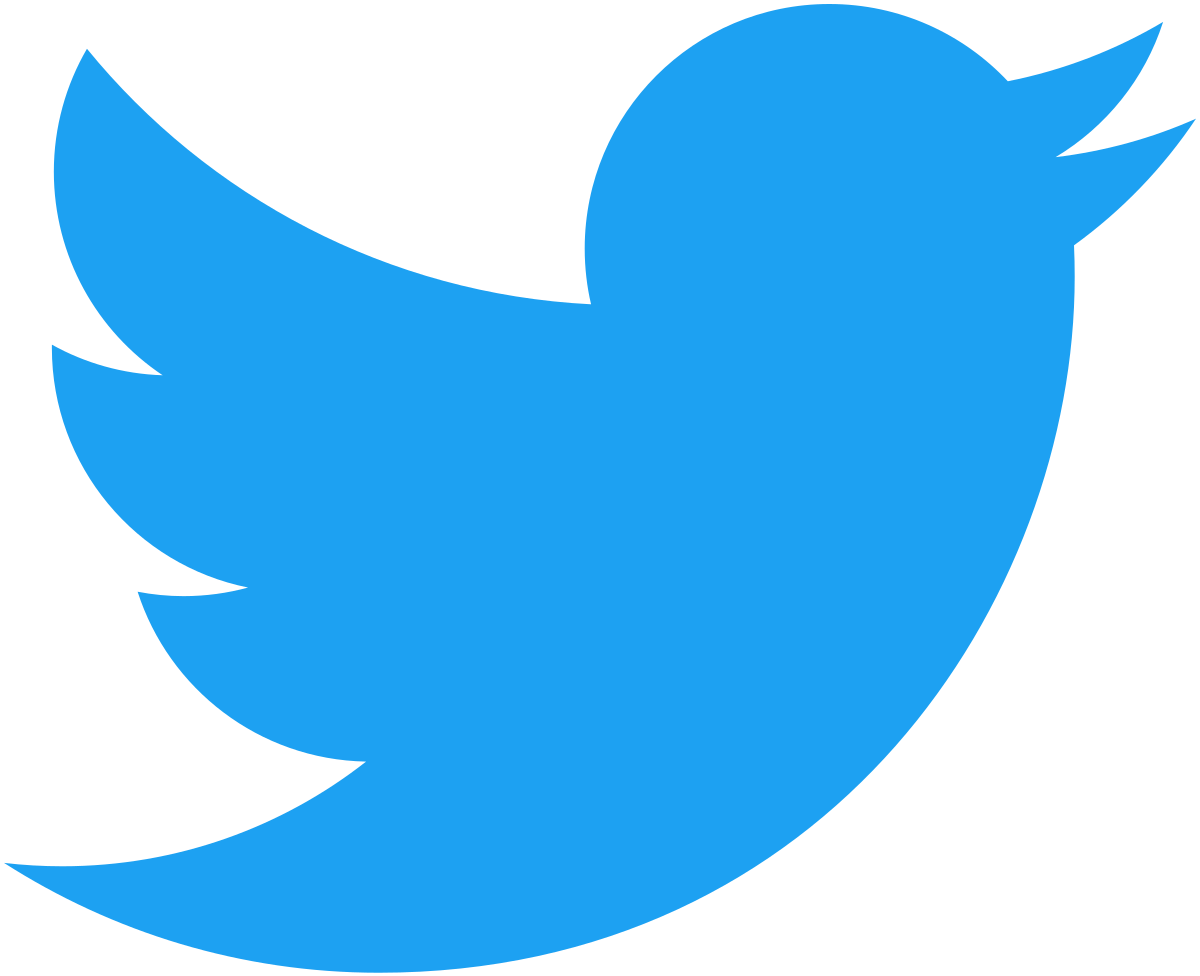
\includegraphics[scale=0.007]{./img/tw_logo.png}   & \begin{tabular}[c]{@{}cl@{}} \href{https://help.twitter.com/en/rules-and-policies/medical-misinformation-policy}{help.twitter.com/en/rules-and-policies/medical-misinformation-policy} \\  \href{https://blog.twitter.com/en\_us/topics/company/2021/updates-to-our-work-on-covid-19-vaccine-misinformation}{blog.twitter.com/en\_us/topics/company/2021/updates-to-our-work-on-covid-19-vaccine-misinformation} \\  \href{https://blog.twitter.com/en\_us/topics/company/2020/covid-19}{blog.twitter.com/en\_us/topics/company/2020/covid-19}\end{tabular}      \\ \cline{2-3} 
                                           & 
\includegraphics[scale=0.03]{./img/yt_logo.png}  & \href{https://support.google.com/youtube/answer/9891785}{support.google.com/youtube/answer/9891785}                                 \\ \hline
\multirow{3}{*}{\begin{tabular}[c]{@{}cl@{}}  Fact-checking \\ policy \end{tabular}} & \includegraphics[scale=0.05]{./img/fb_logo.png} & \href{https://www.facebook.com/journalismproject/programs/third-party-fact-checking/how-it-works}{facebook.com/journalismproject/programs/third-party-fact-checking/how-it-works}                                    \\ \cline{2-3} 
                                           & \includegraphics[scale=0.007]{./img/tw_logo.png}   & x       \\ \cline{2-3} 
                                           & \includegraphics[scale=0.03]{./img/yt_logo.png}  & \href{https://support.google.com/youtube/answer/9229632}{support.google.com/youtube/answer/9229632}                                  \\ \hline
\multirow{3}{*}{\begin{tabular}[c]{@{}cl@{}}  Fighting \\ misinformation \end{tabular}} & \includegraphics[scale=0.05]{./img/fb_logo.png} & \begin{tabular}[c]{@{}cl@{}} \href{https://www.facebook.com/formedia/blog/working-to-stop-misinformation-and-false-news}{facebook.com/formedia/blog/working-to-stop-misinformation-and-false-news}     \\ \href{https://about.fb.com/news/2018/05/hard-questions-false-news/}{about.fb.com/news/2018/05/hard-questions-false-news/}   \end{tabular}                            \\ \cline{2-3} 
                                           & \includegraphics[scale=0.007]{./img/tw_logo.png}   &        \\ \cline{2-3} 
                                           & \includegraphics[scale=0.03]{./img/yt_logo.png}  & \begin{tabular}[c]{@{}cl@{}}  \href{https://www.youtube.com/intl/en\_us/howyoutubeworks/our-commitments/fighting-misinformation/\#policies}{youtube.com/intl/en\_us/howyoutubeworks/our-commitments/fighting-misinformation/\#policies}  \\ \href{https://blog.youtube/inside-youtube/the-four-rs-of-responsibility-raise-and-reduce/}{blog.youtube/inside-youtube/the-four-rs-of-responsibility-raise-and-reduce/}    \end{tabular}                            \\ \hline
                                           
% 

\multirow{3}{*}{\begin{tabular}[c]{@{}cl@{}} Strike System \end{tabular}} & \includegraphics[scale=0.05]{./img/fb_logo.png} & \begin{tabular}[c]{@{}cl@{}} See in the following link the section {\it What is the number of strikes a person or } \\ { \it Page has to get to before you ban them?} \\  \href{https://about.fb.com/news/2018/08/enforcing-our-community-standards/}{about.fb.com/news/2018/08/enforcing-our-community-standards/}   \end{tabular}                            \\ \cline{2-3} 
                                           & \includegraphics[scale=0.007]{./img/tw_logo.png}   &  \begin{tabular}[c]{@{}cl@{}}  See in the following links the section:  {\it Account locks and permanent suspension }   \\ \href{https://help.twitter.com/en/rules-and-policies/election-integrity-policy}{help.twitter.com/en/rules-and-policies/election-integrity-policy}  \\ \href{https://help.twitter.com/en/rules-and-policies/medical-misinformation-policy}{help.twitter.com/en/rules-and-policies/medical-misinformation-policy}  \end{tabular}    \\ \cline{2-3} 
                                           & \includegraphics[scale=0.03]{./img/yt_logo.png}  & \begin{tabular}[c]{@{}cl@{}}  \href{https://support.google.com/youtube/answer/2802032?hl=en. Accessed 21 6 2021}{https://support.google.com/youtube/answer/2802032?hl=en. Accessed 21 6 2021}   \end{tabular}                            \\ \hline 

% 

\multirow{3}{*}{\begin{tabular}[c]{@{}cl@{}} Account suspension \end{tabular}} & \includegraphics[scale=0.05]{./img/fb_logo.png} & \begin{tabular}[c]{@{}cl@{}}    \end{tabular}                            \\ \cline{2-3} 
                                           & \includegraphics[scale=0.007]{./img/tw_logo.png}   &  \begin{tabular}[c]{@{}cl@{}} \href{https://help.twitter.com/en/managing-your-account/suspended-twitter-accounts}{https://help.twitter.com/en/managing-your-account/suspended-twitter-accounts }    \end{tabular}    \\ \cline{2-3} 
                                           & \includegraphics[scale=0.03]{./img/yt_logo.png}  & \begin{tabular}[c]{@{}cl@{}}    \end{tabular}                            \\ \hline                                            

% 

\multirow{3}{*}{\begin{tabular}[c]{@{}cl@{}} Flags, Notice \\ and Information Panels \end{tabular}} & \includegraphics[scale=0.05]{./img/fb_logo.png} & \begin{tabular}[c]{@{}cl@{}}  \href{https://www.facebook.com/business/help/341102040382165}{https://www.facebook.com/business/help/341102040382165}   \end{tabular}                            \\ \cline{2-3} 
                                           & \includegraphics[scale=0.007]{./img/tw_logo.png}   &  \begin{tabular}[c]{@{}cl@{}} \href{https://help.twitter.com/en/rules-and-policies/notices-on-twitter}{https://help.twitter.com/en/rules-and-policies/notices-on-twitter}    \end{tabular}    \\ \cline{2-3} 
                                           & \includegraphics[scale=0.03]{./img/yt_logo.png}  & \begin{tabular}[c]{@{}cl@{}}   \href{https://support.google.com/youtube/answer/9004474?hl=en}{support.google.com/youtube/answer/9004474?hl=en}  \end{tabular}                            \\ \hline
                                                                                  
 \end{tabular}
\caption{Summary of ressources, last accessed on July 5, 2021. }
\label{summary}
\end{table}

\end{landscape}
%https://www.facebook.com/journalismproject/programs/third-party-fact-checking/how-it-works
\end{document}
